\documentclass[a4paper,10pt]{report}
\newcommand{\pmatrice}[1]{\begin{pmatrix}#1\end{pmatrix}}
\usepackage{cours}
\usepackage{pifont}

\begin{document}
\everymath{\displaystyle}
\begin{center}
\textit{{ {\huge TD 11 : Espaces probabilisés}}}
\end{center}

\bigskip


\begin{center}
\textit{{ {\large Dénombrement et dénombrabilité}}}
\end{center}

\medskip

\begin{Exercice}{} Calculer les sommes suivantes ($n \in \mathbb{N}$) : 
$$\dis\sum_{k=0}^n k \binom{n}{k}, \; \dis\sum_{k=0}^n\dis\frac{1}{k+1} \binom{n}{k} \; \hbox{ et } \; \sum_{k=0}^n \binom{2n+1}{k}$$
\end{Exercice}

\corr Soit $f : \mathbb{R} \rightarrow \mathbb{R}$ définie par :
$$ \forall x \in \mathbb{R}, \; f(x)=(x+1)^n = \sum_{k=0}^n \binom{n}{k} x^k$$
La fonction $f$ est dérivable sur $\mathbb{R}$ et on a pour tout réel $x$,
$$ f'(x) = n(1+x)^{n-1}=  \sum_{k=0}^n \binom{n}{k} k x^{k-1} $$
En évaluant en $1$, on obtient :
$$ \sum_{k=0}^n k \binom{n}{k}  = n2^{n-1}$$
En intégrant $f$ sur $[0,1]$, on obtient maintenant :
\begin{align*}
\int_0^1 (1+x)^n \dx & = \int_0^1 \left( \sum_{k=0}^n \binom{n}{k} x^k \right) \dx \\
& = \sum_{k=0}^n \binom{n}{k} \int_0^1 x^k \dx \\
& = \sum_{k=0}^n \binom{n}{k} \dfrac{1}{k+1}
\end{align*}
On a de plus :
$$ \int_0^1 (1+x)^n \dx  = \left[ \dfrac{(1+x)^{n+1}}{n+1} \right]_0^1 = \dfrac{2^{n+1}-1}{n+1}$$
Ainsi,
$$ \sum_{k=0}^n \binom{n}{k} \dfrac{1}{k+1} = \dfrac{2^{n+1}-1}{n+1}$$
Déterminons la troisième somme (notons la $S$). On a :
\begin{align*}
S & = \sum_{k=0}^{n} \binom{2n+1}{k} \\
& = \sum_{k=0}^{n} \binom{2n+1}{2n+1-k} \\
& = \binom{2n+1}{2n+1} + \binom{2n+1}{2n} + \cdots + \binom{2n+1}{n+1} \\
& = \sum_{k=n+1}^{2n+1} \binom{2n+1}{k}
\end{align*}
On en déduit alors que :
\begin{align*}
2S &  = \sum_{k=0}^{n} \binom{2n+1}{k} + \sum_{k=n+1}^{2n+1} \binom{2n+1}{k} \\
& = \sum_{k=0}^{2n+1} \binom{2n+1}{k} \\
& = (1+1)^{2n+1} \\
& = 2^{2n+1} 
\end{align*}
et ainsi :
$$  S= 2^{2n} = 4^n $$

\begin{Exercice}{} Soit $(p, n) \in \mathbb{N}^2$ tel que $p \leq n$. Déterminer la valeur de $\dis\sum_{k=p}^n{k\choose p} \cdot$

%={n+1\choose p+1}\cdot$
\end{Exercice}

\corr Notons $S$ cette somme. On a :
\begin{align*}
S & = \binom{p}{p} + \binom{p+1}{p} + \binom{p+2}{p} + \cdots + \binom{n}{p} \\
& = \binom{p+1}{p+1} + \binom{p+1}{p} + \binom{p+2}{p} + \cdots + \binom{n}{p} \\
& =  \binom{p+2}{p+1} + \binom{p+2}{p} + \cdots + \binom{n}{p} 
\end{align*}
d'après la formule de Pascal. En la réutilisant, on a :
$$ S = \binom{p+3}{p+1} +  \cdots + \binom{n}{p} $$
De proche en proche, on obtient :
$$ S = \binom{n}{p+1}  + \binom{n}{p} = \binom{n+1}{p+1} $$

\begin{Exercice}{}Soient $3$ urnes $U_1,U_2$ et $U_3$ et $n$ boules numérotées ($n \in \mathbb{N}^*$) de 1 à $n$.
\begin{enumerate}
\item Quel est le nombre total de répartitions de ces boules dans les trois urnes ?
\item Quel est le nombre total de répartitions qui laissent au moins $U_1$ vide ? au moins une urne vide ?
\item En déduire le nombre de répartitions qui ne laissent aucune urne vide.
\end{enumerate}
\end{Exercice}

\corr 

\begin{enumerate}
\item Pour chacune des $n$ boules, il y a $3$ choix d'urnes possibles donc il y a $3^n$ répartitions possibles.
\item Pour laisser $U_1$ vide, il reste deux choix d'urnes pour chacune des $n$ boules donc il y a $2^n$ répartitions possibles. Pour laisser au moins une urne vide, on peut laisser $U_1$ vide ($2^n$ répartitions), ou $U_2$  ($2^n$ répartitions), ou $U_3$  ($2^n$ répartitions). Dans ces répartitions, on a compté deux fois les répartitions qui laissaient deux urnes vides (il y en a $3$ qui correspondent aux répartitions où on remplit uniquement une urne). Ainsi, il y a $3 \times 2^n - 3$ répartitions qui laissent au moins une urne vide.
\item Il y a $3^n$ répartitions en tout et $3 \times 2^n - 3$ répartitions qui laissent au moins une urne vide donc il y a :
$$ 3^n - (3 \times 2^n - 3) = 3^n - 3 \times 2^n + 3$$
répartitions qui ne laissent aucune urne vide.
\end{enumerate}

\begin{Exercice}{} Un tiroir contient 5 paires de chaussures noires, 3 paires de chaussures vertes et 2 paires de chaussures rouges. Toutes les paires d'une même couleur ont des formes différentes. On prend deux chaussures au hasard simultanément dans le tiroir.
\begin{enumerate}
\item Combien y a-t-il de tirages possibles ?
\item 
Combien de tirages donnent :
\begin{enumerate}
\item deux chaussures de même couleur ?
\item un pied gauche et un pied droit ?
\item au moins un pied gauche ?
\item deux chaussures de la même couleur avec un pied gauche et un pied droit ?
\item une vraie paire de chaussures (deux chaussures de même couleur et même forme avec un pied gauche et un pied droit) ?
\end{enumerate}
\end{enumerate}
\end{Exercice}

\corr 
\begin{enumerate}
\item Cela revient à dénombrer le nombre d'ensemble à deux éléments dans un ensemble à $20$ éléments. Ainsi, il y a :
$$ \binom{20}{2} = \dfrac{20\times 19}{2} = 190$$
tirages possibles. 
\item \begin{enumerate}
\item On distingue trois cas deux à deux distincts :
\begin{itemize}
\item Il y a $\binom{10}{2}$ tirages avec deux chaussures noires.
\item Il y a $\binom{6}{2}$ tirages avec deux chaussures vertes.
\item Il y a $\binom{4}{2}$ tirages avec deux chaussures rouges.
\end{itemize}
Ainsi, il y a :
$$ \binom{10}{2} + \binom{6}{2} + \binom{4}{2} = 45+ 15+6=66$$
tirages avec deux chaussures de la même couleur.
\item Il y a $10$ pieds gauches et $10$ pieds droits. Il y a donc $10$ choix pour chacun des pieds donc il y a $10^2=100$ tirages avec un pied gauche et un pied droit.
\item Le nombre de tirages avec au moins un pied gauche est égal au nombre de tirages total auquel on soustrait le nombre de tirages avec deux pieds droits. Dénombrer le nombre de tirages avec deux pieds droits revient à déterminer le nombre d'ensembles à deux éléments dans un ensemble à $10$ éléments : il y en a donc $\binom{10}{2}=45$. Ainsi, il y a :
$$ 190 - 45= 145$$
tirages avec au moins un pied gauche. 
\item On distingue trois cas deux à deux distincts.
\begin{itemize}
\item Pour dénombrer le nombre de tirages avec deux chaussures noires, avec un pied gauche et un pied droit, on a $5$ choix pour le pied gauche et $5$ choix pour le pied droit donc il y a $25$ tirages correspondant.
\item Pour dénombrer le nombre de tirages avec deux chaussures vertes, avec un pied gauche et un pied droit, on a $3$ choix pour le pied gauche et $3$ choix pour le pied droit donc il y a $9$ tirages correspondant.
\item Pour dénombrer le nombre de tirages avec deux chaussures rouges, avec un pied gauche et un pied droit, on a $2$ choix pour le pied gauche et $2$ choix pour le pied droit donc il y a $4$ tirages correspondant.
\end{itemize}
Ainsi, on a :
$$ 25+9+4 = 38$$
tirages avec deux chaussures de la même couleur avec un pied gauche et un pied droit.
\item Il y a $10$ vraies paires de chaussures donc il y a $10$ tirages correspondants.
\end{enumerate}
\end{enumerate}

\begin{Exercice}{} Soit $f : \mathbb{N}^2 \rightarrow \mathbb{N}$ définie par :
$$ f((p,q)) = \frac{(p+q)(p+q+1)}{2} + q$$
\begin{enumerate}
\item Calculer $f((0,0))$, $f((1,0))$, $f((0,1))$, $f((2,0))$ et $f((1,1))$.
\item Représenter sur un schéma la manière dont $f$ liste les éléments de $\mathbb{N}^2$.
\item Nous souhaitons montrer que $\mathbb{N}^2$ est dénombrable. 
\begin{enumerate}
\item Soit $n \geq 0$. Justifier l'existence de :
$$ m_0 = \max \left\lbrace m \geq 0, \, \frac{m(m+1)}{2} \leq n \right\rbrace$$
Encadrer alors $n-\dfrac{m_0(m_0+1)}{2}$ et en déduire que $f$ est une surjection de $\mathbb{N}^2$ sur $\mathbb{N}$.
\item Montrer que $f$ est injective.
\item Conclure.
\end{enumerate}
\end{enumerate}
\end{Exercice}

\corr 
\begin{enumerate}
\item On a :
$$ f((0,0)) = 0,f((1,0))=1, f((0,1))= 2, f((2,0))=3 \; \hbox{ et } f((1,1))=4$$

\item Voici un tel schéma : 

\begin{center}
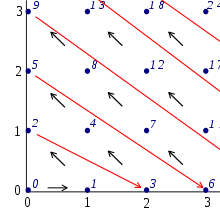
\includegraphics[scale=0.5]{den}
\end{center}

\item 
\begin{enumerate}
\item Soit $n \geq 0$. Notons $A_n$ l'ensemble défini par :
$$ A_n = \left\lbrace m \geq 0, \, \frac{m(m+1)}{2} \leq n \right\rbrace = \left\lbrace m \geq 0, \, 0+1+2+ \cdots + m \leq n \right\rbrace$$
Alors $A_n$ est un sous-ensemble de $\mathbb{N}$, non vide car $0$ appartient à cet ensemble et il est majoré par $n$ car si $m$ appartient à $A_n$ :
$$ m \leq 0+1+ \cdots + m \leq n$$
Ainsi, $A_n$ admet un plus grand élément et on pose :
$$ m_0 = \max \left\lbrace m \geq 0, \, \frac{m(m+1)}{2} \leq n \right\rbrace$$
Sachant que $m_0$ est le plus grand élément de $A_n$, on en déduit que $m_0+1$ n'appartient pas à $A_n$ donc :
$$ \frac{(m_0+1)(m_0+2)}{2} > n$$
et ainsi par définition de $m_0$ :
$$ \frac{m_0(m_0+1)}{2} \leq n  <\frac{(m_0+1)(m_0+2)}{2}$$
donc :
$$   0 \leq  n- \frac{m_0(m_0+1)}{2} <\frac{(m_0+1)(m_0+2)}{2} - \frac{m_0(m_0+1)}{2}$$
On a :
\begin{align*}
\frac{(m_0+1)(m_0+2)}{2} - \frac{m_0(m_0+1)}{2} & = \dfrac{m_0+1}{2} ((m_0+2)-m_0) \\
& = m_0+1 
\end{align*}
On en déduit qu'il existe un entier $k \in \Interv{0}{m_0}$ tel que :
$$ n = \frac{m_0(m_0+1)}{2} + k$$
et ainsi (remarquons que $m_0-k \in \mathbb{N}$) : 
$$ n = f(m_0-k,k)$$
Ainsi, pour tout entier $n \in \mathbb{N}$, il existe un couple d'entiers $(p,q)$ tel que $n=f(p,q)$. On en déduit que $f$ est une surjection de $\mathbb{N}^2$ sur $\mathbb{N}$.
\item Soient $(p,q)$ et $(p',q')$ deux couples d'entiers tels que :
$$ f((p,q))=f((p',q'))$$
Alors :
$$ 1+2+ \cdots + (p+q) + q = 1+2+ \cdots + (p'+q') + q'$$
Supposons que $p+q<p'+q'$. Alors :
$$ q= (p+q+1)+ \cdots +(p'+q') + q'$$
C'est absurde car :
$$ (p+q+1)+ \cdots +(p'+q') + q' \geq (p'+q')+q' \geq p'+q'>p+q \geq q$$
On a donc $p+q \geq p'+q'$. On montre de même que $p+q \leq p'+q'$ et ainsi :
$$ p+q = p'+q'$$
On sait que :
$$  1+2+ \cdots + (p+q) + q = 1+2+ \cdots + (p'+q') + q'$$
donc $q=q'$ et ainsi $p=p'$ et finalement $(p,q)=(p',q')$. Ainsi, $f$ est injective.
\item On en déduit que $f$ est une bijection de $\mathbb{N}^2$ sur $\mathbb{N}$ donc $\mathbb{N}^2$ est dénombrable.
\end{enumerate}
\end{enumerate}




\medskip

\begin{center}
\textit{{ {\large Équiprobabilité}}}
\end{center}

\medskip



\begin{Exercice}{} Un jeu de cartes comporte $32$ cartes. On tire simultanément $8$ cartes dans ce jeu de $32$ cartes. 

\begin{enumerate}
\item Quelle est la probabilité d'obtenir au moins un pique ?
\item Quelle est la probabilité d'obtenir exactement un pique ?
\item Quelle est la probabilité d'obtenir 2 carrés (un carré est constitué de 4 cartes de la même hauteur, par exemple 4 rois)?
\item Quelle est la probabilité d'obtenir un roi et un pique exactement ?
\end{enumerate}
\end{Exercice} 

\corr Nous sommes en situation d'équiprobabilité. L'univers $\Omega$ contient $\dis \binom{32}{8}$ issues : en effet, on tire \textit{simultanément} 8 cartes dans un jeu de 32 cartes.

\begin{enumerate}
\item Soit $A$ l'évènement \og On obtient au moins un pique \fg$\cdot$ L'évènement $\overline{A}$ est \og On obtient aucun pique \fg $\cdot$ On a alors Card$(\overline{A}$)=$\dis \binom{24}{8}$ (car l'évènement est realisé si on tire simultanément $8$ cartes parmi les cartes que ne sont pas des piques, c'est-à-dire $24$ cartes). On a alors :
\[ P(\overline{A}) = \frac{\hbox{Card}(\overline{A})}{\hbox{Card}(\Omega)} = \frac{\binom{24}{8}}{\binom{32}{8}}\]
et ainsi :
\[ P(A) = 1 - P(\overline{A}) = 1 - \frac{\binom{24}{8}}{\binom{32}{8}}  \]

\item Soit $B$ l'évènement \og On obtient exactement un pique \fg$\cdot$ Pour obtenir exactement un pique, on doit tirer un pique parmi les huit possibles et $7$ cartes parmi les $24$ cartes qui ne sont pas des piques. Ainsi :
\[ \hbox{Card}(B) = \binom{8}{1} \binom{24}{7} = 8 \binom{24}{7} \]
donc :
\[ P(B) = \dis \frac{\hbox{Card}(B)}{\hbox{Card}(\Omega)} = \frac{8\binom{24}{7}}{\binom{32}{8}} \]

\item Soit $C$ l'évènement \og On obtient deux carrés \fg$\cdot$ Il y a $8$ carrés possibles, il y a donc $\dis \binom{8}{2}$ manières d'obtenir $2$ carrés. Ainsi :
\[ \hbox{Card}(C) = \binom{8}{2} \]
donc :
\[ P(C)= \frac{\hbox{Card}(C)}{\hbox{Card}(\Omega)} = \frac{\binom{8}{2}}{\binom{32}{8}}\]

\item Soit $D$ l'évènement \og On obtient un roi et un pique exactement \fg$\cdot$ Pour obtenir un roi et un pique exactement, on distingue deux cas :
\begin{itemize}
\item On peut obtenir le roi de pique et $7$ cartes parmi les cartes qui ne sont pas des rois ou des piques (il y en $21$ : $32$ cartes au total auquel on enlève les $8$ piques et les trois rois non piques). Il y a $\dis \binom{1}{1}\binom{21}{7}=\binom{21}{7}$ tirages possibles dans ce cas.
\item On peut obtenir un roi non pique, un pique parmi les sept possibles (non roi) et $6$ cartes parmi les cartes qui ne sont pas des rois et des piques. Il y a $\dis \binom{3}{1} \binom{7}{1} \binom{21}{6}= 3 \times 7  \binom{21}{6}$ tirages possibles dans ce cas.
\end{itemize}
On a ainsi :
\[ \hbox{Card}(D) = \binom{21}{7} + 21 \binom{21}{6}\]
donc :
\[  P(D)= \frac{\hbox{Card}(D)}{\hbox{Card}(\Omega)} = \frac{\binom{21}{7} + 21 \binom{21}{6}}{\binom{32}{8}}\]
\end{enumerate}

\begin{Exercice}{Le problème des anniversaires}
On considère un groupe de $n$ personnes ($n \in \mathbb{N}^*$ avec $n \leq 365$).\\
Quelle est la probabilité qu'au moins deux personnes aient leur anniversaire le même jour ?
\end{Exercice}

\corr En considérant cette expérience comme une expérience aléatoire et en considérant que l'on est en situation d'équiprobabilité, on peut modéliser celle-ci avec l'univers $\Omega$ constitué de $n$-listes formées de dates d'anniversaire ($365$ choix). Ainsi,
$$ \textrm{Card}(\Omega) = 365^n$$
Soit $A$ l'évènement défini par :

\begin{center}
$A$ : \og Au moins deux personnes ont leur anniversaire le même jour \fg{} 
\end{center}
On a alors :
\begin{center}
$\overline{A}$ : \og Les membres du groupe ont tous une date d'anniversaire différente \fg{} 
\end{center}
Une issue de $\overline{A}$ est une liste d'éléments distincts de $\Omega$ donc :
$$ \textrm{Card}(\overline{A}) = 365 \times 364 \times \cdots \times (365-(n-1)) = \dfrac{365!}{(365-n)!}$$
On en déduit que :
$$ P(\overline{A}) = \dfrac{\dfrac{365!}{(365-n)!}}{365^n}$$
et ainsi :
$$ P(A) = 1- P(\overline{A}) = 1 - \dfrac{\dfrac{365!}{(365-n)!}}{365^n}$$


\begin{Exercice}{} Une urne contient 5 boules blanches et 10 boules noires.

\begin{enumerate}
\item On tire au hasard successivement et avec remise 2 boules de l'urne.
\begin{enumerate}
\item Quelle est la probabilité d'obtenir une boule blanche et une boule noire dans cet ordre ?
\item Quelle est la probabilité d'obtenir une boule blanche et une boule noire dans un ordre quelconque ?
\end{enumerate}
\item Mêmes questions dans le cas de tirages sans remise.
\item On tire simultanément 5 boules de l'urne. Quelle est la probabilité d'obtenir 2 boules blanches et 3 boules noires ?
\end{enumerate}
\end{Exercice}

\corr 

\begin{enumerate}
\item Une issue de l'expérience aléatoire est une liste à deux éléments d'un ensemble à $15$ éléments. En notant $\Omega$ l'univers, on a :
$$ \textrm{Card}(\Omega)= 15^2$$
Nous sommes en situation d'équiprobabilité.

\begin{enumerate}
\item Soit $A$ cet évènement. Il y a $5$ boules blanches et $10$ boules noires donc :
$$ \textrm{Card}(A)= 5 \times 10 = 50$$
et ainsi,
$$ \P(A) = \dfrac{\textrm{Card}(A)}{\textrm{Card}(\Omega)} = \dfrac{50}{15^2}$$
\item Soit $B$ cet évènement. Remarquons que $B$ est l'union disjointe de $A$ et de $C$ : \og On obtient une boule noire et une boule blanche dans cet ordre \fg. De la même manière que dans la question précédente, on montre que :
$$ \P(C) = \dfrac{50}{15^2}$$
Ainsi, par incompatibilité :
$$ \P(B) = \P(A)+ \P(C) = \dfrac{100}{15^2}$$
\end{enumerate}
\item Seul le cardinal de l'univers change : 
$$ \textrm{Card}(\Omega)= 15 \times 14$$
Les cardinaux de $B$ et $C$ restent les mêmes. On obtient :
$$ \P(A)   = \dfrac{50}{15 \times 14}$$
et 
$$ \P(B)   = \dfrac{100}{15 \times 14}$$
\item Une issue de l'expérience aléatoire est un sous-ensemble à $5$ éléments de l'ensemble des boules. Ainsi,
$$ \textrm{Card}(\Omega)= \binom{15}{5} $$
Soit $D$ l'évènement \og On obtient 2 boules blanches et 3 boules noires \fg. L'évènement $D$ se réalise si et seulement on obtient deux boules blanches parmi les $5$ et $3$ boules noires parmi les $10$ donc :
$$ \textrm{Card}(D) = \binom{5}{2} \binom{10}{3}$$
Nous sommes en situation d'équiprobabilité donc :
$$ \P(D) = \dfrac{\binom{5}{2} \binom{10}{3}}{\binom{15}{5}}$$
\end{enumerate}

\newpage


\medskip

\begin{center}
\textit{{ {\large Tribu et probabilité}}}
\end{center}

\medskip


\begin{Exercice}{} Soit $\Omega$ un univers muni d'une tribu ${\cal A}$. On se donne un sous-ensemble $\Omega'$ de $\Omega$ et on pose :
 $${\cal A}'=\{A\cap \Omega',\ A\in{\cal A}\}$$
Montrer que ${\cal A}'$ est une tribu sur $\Omega'.$
\end{Exercice}

\corr Montrons les trois points de la définition d'une tribu.

\begin{itemize}
\item $\mathcal{A}$ est une tribu sur $\Omega$ donc $\Omega \in \mathcal{A}$ donc par définition de $\mathcal{A}'$, $ \Omega \cap \Omega' \in \mathcal{A}'$. Or $\Omega' \subset \Omega$ donc $ \Omega \cap \Omega' = \Omega'$ et ainsi $\Omega' \in \mathcal{A}'$.
\item Soit $B \in \mathcal{A}'$. Montrons que $\Omega' \setminus B \in \mathcal{A}'$. Par définition de $\mathcal{A}'$, il existe $A \in \mathcal{A}$ tel que :
$$ B = A \cap \Omega'$$
Ainsi,
$$ \Omega' \setminus B  = \Omega' \setminus  (A \cap \Omega') $$
Or les éléments de $\Omega' \setminus  (A \cap \Omega')$ sont les éléments de $\Omega'$ qui n'appartiennent pas à $A \cap \Omega'$ donc ce sont tout simplement les éléments de $\Omega'$ qui ne sont pas dans $A$. Ainsi,
$$  \Omega' \setminus B = \Omega' \setminus A = \Omega' \cap \overline{A}$$
On sait que $A \in \mathcal{A}$ donc par stabilité par passage au complémentaire, on a $\overline{A} \in \mathcal{A}$. Ainsi, par définition de $\mathcal{A}'$, on en déduit que $\Omega' \setminus B \in \mathcal{A}'$.
\item Soit $(A_n)_{n \geq 0}$ une famille d'évènements de $\mathcal{A}'$. Pour tout entier $n \geq 0$, il existe un évènement $B_n \in \mathcal{A}$ tel que :
$$ A_n = B_n \cap \Omega$$
Ainsi,
\begin{align*}
\bigcup_{n=0}^{+ \infty} A_n & = \bigcup_{n=0}^{+ \infty}B_n \cap \Omega \\
& = \left( \bigcup_{n=0}^{+ \infty}B_n \right) \cap \Omega
\end{align*}
Pour tout entier $n \geq 0$, $B_n \in \mathcal{A}$ donc par stabilité par réunion dénombrable $(\mathcal{A}$ est une tribu),
$$  \bigcup_{n=0}^{+ \infty}B_n \in \mathcal{A}$$
et par définition de $\mathcal{A}'$, on en déduit que :
$$ \bigcup_{n=0}^{+ \infty} A_n \in \mathcal{A}'$$
\end{itemize}
Ainsi, $\mathcal{A}'$ est une tribu de $\Omega'$.

\begin{Exercice}{}  Soient $E,F$ deux évènements d'un même espace probabilisé.
\begin{enumerate}
\item Montrer que $P(E \cup F) \leq P(E) + P(F)$.
\item Soit $G$ un évènement. Montrer que $P(E \cup F \cup G) \leq P(E) + P(F) + P(G)$.
\item Écrire cette inégalité pour $\overline{E}$, $\overline{F}$ et $\overline{G}$ et en déduire que si $E,F$ et $G$ sont équiprobables de probabilité $p$ et si $P(E \cap F \cap G)=0$ alors $p \leq \dis \frac{2}{3} \cdot$
\end{enumerate}
\end{Exercice}

\corr 
\begin{enumerate}
\item On a :
$$ P(E \cup F) = P(E) + P(F) - P(E \cap F) \leq P(E)+P(F)$$
car $P(E \cap F) \geq 0$.
\item On utilise deux fois le résultat de la question précédente :
\begin{align*}
P(E \cup F \cup G) & = P((E \cup F) \cup G) \\
& \leq P(E \cup F) + P(G) \\
& \leq P(E) + P(F) + P(G)
\end{align*}
\item D'après la question précédente,
$$ P(\overline{E} \cup \overline{F} \cup \overline{G})  \leq  P(\overline{E}) + P(\overline{F}) + P(\overline{G})$$
donc d'après les lois de Morgan :
$$ P(\overline{E \cap F \cap G}) \leq 3-P(E)-P(F)-P(G)$$
puis :
$$ 1-P(E \cap F \cap G) \leq 3-3p$$
D'après l'hypothèse, on a $P(E \cap F \cap G)=0$ donc :
$$ 1 \leq 3-3p$$
et ainsi :
$$3p \leq 2$$
et finalement :
$$ p \leq \dfrac{2}{3}$$
\end{enumerate}


\begin{Exercice}{} Soient $n \geq 1$ et $(A_1, \ldots, A_n)$ une famille de $n$ évènements d'un espace probabilisé $(\Omega, \mathcal{A}, \P)$. Montrer que :
$$ \P(A_1 \cup \cdots \cup A_n) \leq \P(A_1) + \cdots + \P(A_n) \leq P(A_1 \cap \cdots \cap A_n) + n-1$$
\end{Exercice}

\corr Montrons les deux inégalités par récurrence.

\medskip

\noindent Pour tout entier $n \geq 1$, on définit la propriété $\mathcal{P}(n)$ par : pour toute famille de $n$ évènements $(A_1, \ldots, A_n)$ de $(\Omega, \mathcal{A}, \P)$, 
$$ \P(A_1 \cup \cdots \cup A_n) \leq \P(A_1) + \cdots + \P(A_n) \leq P(A_1 \cap \cdots \cap A_n) + n-1$$

\begin{itemize}
\item La propriété est vraie au rang $1$ car dans ce cas, pour tout événement $A_1$, les trois quantités sont égales à $P(A_1)$.
\item Soit $n \in \mathbb{N}^*$ tel que $\mathcal{P}(n)$ soit vraie. Soit $(A_1, \ldots, A_{n+1})$ une famille d'événements. On a :
\begin{align*}
\P(A_1 \cup \cdots \cup A_n \cup A_{n+1}) & = \P(A_1 \cup \cdots  \cup A_{n}) + \P(A_{n+1}) - \P((A_1 \cup \cdots \cup A_n) \cap A_{n+1}) \\
& \leq \P(A_1 \cup \cdots  \cup A_{n}) + \P(A_{n+1}) \quad \hbox{ car } \P((A_1 \cup \cdots \cup A_n) \cap A_{n+1}) \geq 0 \\
& \leq \P(A_1) + \cdots + \P(A_n) + \P(A_{n+1})
\end{align*}
d'après l'hypothèse de récurrence. On a donc démontré l'inégalité \og de gauche \fg.

\medskip

\noindent D'après l'hypothèse de récurrence, on a :
$$  \P(A_1) + \cdots \P(A_n) + \P(A_{n+1}) \leq P(A_1 \cap \cdots \cap A_n) + n-1  + \P(A_{n+1})$$
D'après la formule des probabilités totales, en utilisant le système complet d'évènements $(A_{n+1}, \overline{A_{n+1}})$, on a :
$$ P(A_1 \cap \cdots \cap A_n) = P(A_1 \cap \cdots \cap A_n \cap A_{n+1}) + P(A_1 \cap \cdots \cap A_n \cap \overline{A_{n+1}})$$
Ainsi,
$$ \P(A_1) + \cdots \P(A_n) + \P(A_{n+1}) \leq P(A_1 \cap \cdots \cap A_n \cap A_{n+1}) + P(A_1 \cap \cdots \cap A_n \cap \overline{A_{n+1}}) + n-1  + \P(A_{n+1})$$
Or on sait que :
$$ A_1 \cap \cdots \cap A_n \cap \overline{A_{n+1}} \subset \overline{A_{n+1}}$$
donc par croissance :
$$ \P(A_1 \cap \cdots \cap A_n \cap \overline{A_{n+1}}) \leq \P(\overline{A_{n+1}})$$
On en déduit que : 
$$ \P(A_1) + \cdots \P(A_n) + \P(A_{n+1}) \leq P(A_1 \cap \cdots \cap A_n \cap A_{n+1}) + P(\overline{A_{n+1}}) + n-1  + \P(A_{n+1})$$
Sachant que :
$$ P(\overline{A_{n+1}}) + \P(A_{n+1})=1$$
On en déduit finalement que :
$$  \P(A_1) + \cdots \P(A_n) + \P(A_{n+1}) \leq P(A_1 \cap \cdots \cap A_n \cap A_{n+1}) +n $$
ce qui prouve l'inégalité \og de droite \fg.
\item La propriété est vraie au rang $1$ et est héréditaire. Par principe de récurrence, elle est vraie pour tout entier $n \geq 1$.
\end{itemize}


\begin{Exercice}{} Soit $(a_n)_{n \geq 0}$ une suite strictement décroissante de réels strictement positifs de limite nulle.  Déterminer $\lambda \in \R$ tel qu'il existe une probabilité $\P$ sur $\bigl(\N,\mathcal{P}(\N)\bigr)$ vérifiant :
    \[
    \forall n \geq 0, \qquad \P\bigl( \lbrace n, n+1, \ldots \rbrace) = \lambda a_n
    \]
\end{Exercice} 

\corr Pour tout $n \geq 0$, notons :
$$ A_n = \lbrace n, n+1, \ldots \rbrace$$
Raisonnons par analyse-synthèse.

\medskip

\noindent $\rhd$ \textit{Analyse.} Soit $\lambda \in \mathbb{R}$ vérifiant la propriété de l'énoncé. Alors la série de terme général $\P (\lbrace n \rbrace)$ converge et sa somme vaut $1$. Pour tout $n \geq 0$,
$$ \lbrace n \rbrace = A_n \setminus A_{n+1}$$
donc :
\begin{align*}
 \P (\lbrace n \rbrace) & = \P (A_n) - \P (A_n \cap A_{n+1}) \\
 & = \P (A_n) - \P (A_{n+1}) \\
 & = \lambda a_n - \lambda a_{n+1}
 \end{align*}
Ainsi, pour tout entier $N \geq 0$,
\begin{align*}
\sum_{k=0}^N  \P (\lbrace k \rbrace) & = \sum_{k=0}^N\lambda a_k - \lambda a_{k+1} \\
& = \lambda a_0 - \lambda a_{N+1} 
\end{align*}
On en déduit que (en utilisant que $(a_n)$ converge vers $0$) :
$$ 1 = \sum_{k=0}^{+ \infty}  \P (\lbrace k \rbrace) = \lim_{N \rightarrow + \infty} \sum_{k=0}^N  \P (\lbrace k \rbrace) = \lambda a_0$$
Ainsi, $\lambda$ et $a_0$ sont non nuls et :
$$ \lambda = \dfrac{1}{a_0}$$

\medskip

\noindent $\rhd$ \textit{Synthèse.} Posons :
$$ \lambda = \dfrac{1}{a_0}$$
Les calculs précédents prouvent que la série de terme général $\P( \lbrace n \rbrace)$ converge et que sa somme vaut $1$. Pour tout entier $n \geq 0$,
$$ \P( \lbrace n \rbrace) = \dfrac{1}{a_0} (a_n - a_{n+1}) \geq 0$$
car $(a_n)_{n \geq 0}$ est une suite décroissante positive. Ainsi, avec ce choix de $\lambda$, il existe une probabilité $\P$ sur $\bigl(\N,\mathcal{P}(\N)\bigr)$ vérifiant :
    \[
    \forall n \geq 0, \qquad \P\bigl( \lbrace n, n+1, \ldots \rbrace) = \lambda a_n
    \]
    


\newpage

\medskip

\begin{center}
\textit{{ {\large Probabilités conditionnelles}}}
\end{center}

\medskip

\begin{Exercice}{} On peut distinguer des élèves en trois catégories : ceux qui aiment la chimie, ceux qui n'aiment pas et ceux qui s'en fichent (royalement). Les étudiants des classes PC et PSI du lycée Robespierre sont assez différents : les étudiants en PC aiment la chimie avec une probabilité de $0.6$ et n'aiment pas avec une probabilité de $0.2$ alors que les étudiants en PSI aiment la chimie avec une probabilité de $0.4$ et s'en fichent avec une probabilité de $0.4$. On rencontre un étudiant au hasard et on suppose qu'il a deux fois plus de chance d'être en PSI plutôt qu'en PC.

\begin{enumerate}
\item Quelle est la probabilité qu'il aime la chimie?
\item Si il aime la chimie, quelle est la probabilité qu'il soit en PC?
\end{enumerate}
\end{Exercice}

\corr Soient $E$ l'évènement \og L'étudiant est en PC \fg , $F_1$ l'évènement \og L'étudiant aime la chimie \fg , $F_2$ l'évènement \og L'étudiant n'aime pas la chimie \fg et $F_3$ l'évènement \og L'étudiant se fiche de la chimie \fg $\cdot$

\medskip

\noindent D'après l'énoncé,
$$ P(E) = \dfrac{1}{3} \; \hbox{ et } \; P(\overline{E}) = \dfrac{2}{3}$$
\begin{enumerate}
\item $(E, \overline{E})$ est un système complet d'évènements de probabilités non nulles. D'après la formule des probabilités totales, on a alors :
\[ P(F_1) = P(E) P_E(F_1) + P(\overline{E})P_{\overline{E}}(F_1) \]
et d'après l'énoncé on a donc :
\[ P(F_1) = \dfrac{1}{3} \times 0.6 + \dfrac{2}{3} \times 0.4 = \dfrac{7}{15} \]
\item On cherche $P_{F_1}(E)$. Par définition, on a :
\[ P_{F_1}(E) = \frac{P(E \cap F_1)}{P(F_1)} = \frac{P(E) P_E(F_1)}{P(F_1)} \]
D'après la question précédente et l'énoncé, on a :
\begin{align*}
\P_{F_1}(E) & = \frac{(1/3) \times (6/10)}{7/15} \\
& = \dfrac{1/5}{7/15} \\
& = \dfrac{15}{35} \\
& = \dfrac{3}{7}
\end{align*}
\end{enumerate}

\begin{Exercice}{} On considère deux urnes $U$ et $V$. L'urne $U$ contient 7 boules blanches et 3 boules noires et l'urne $V$ contient 3 boules blanches et 7 boules noires.

\begin{enumerate}
\item Une personne lance un dé parfaitement équilibré 3 fois de suite.\\
 Quelle est la probabilité que la personne obtienne 3 numéros différents les uns des autres ?
\item Une personne lance un dé parfaitement équilibré 3 fois de suite.\\
Si les 3 numéros obtenus sont différents les uns des autres alors elle effectue un tirage d'une boule dans l'urne $U$, sinon elle effectue un tirage d'une boule dans l'urne $V$.
\begin{enumerate}
\item Quelle est la probabilité que la personne obtienne une boule blanche ?
\item Sachant qu'elle a obtenu une boule blanche, quelle est la probabilité que les 3 numéros obtenus aient été distincts ?
\end{enumerate}
\end{enumerate}
\end{Exercice} 

\corr \begin{enumerate}
\item Chaque issue de cette expérience aléatoire correspond à une liste à $3$ éléments de l'ensemble $\{1,2,3,4,5,6\}$ (il y a un ordre et la répétition est possible). Le cardinal de l'univers est donc $6^3$.

\noindent Soit $A$ l'événement \og La personne obtient trois numéros différents les uns des autres \fg $\cdot$

\noindent Une issue réalisant $A$ est une 3-liste avec
\begin{itemize}
 \item 6 possibilités pour le premier numéro;
 \item 5 possibilités pour le deuxième numéro;
 \item 4 possibilités pour le troisième numéro.
\end{itemize}
Il y a donc $6\times 5\times 4$ issues qui réalisent $A$. De plus il s'agit d'une situation d'équiprobabilité car le dé est équilibré donc
$$\P(A) = \frac{6\times 5\times 4}{6^3} = \frac 59$$

\item 
\begin{enumerate}
\item Soit $B$ l'événement \og La personne obtient une boule blanche \fg $\cdot$

\noindent On note toujours $A$ l'événement \og La personne obtient trois numéros différents les uns des autres \fg $\cdot$

\noindent $(A,\overline{A})$ est un système complet d'événements avec $P(A) \neq 0$ et $P(\overline{A}) \neq 0$ donc d'après la formule des probabilités totales, on a :
\begin{align*}
 P(B)&=P(A \cap B)+P(\overline{A} \cap B)\\
 &=P(A)P_{A}(B)+P(\overline{A})P_{\overline{A}}(B)\\
 &=P(A)P_{A}(B)+(1-P(A))P_{\overline{A}}(B).
\end{align*}

\noindent Par équiprobabilité d'un tirage dans l'urne $U$, on a ${P_{A}(B)=\dis \frac 7{10}}\cdot$

\noindent Par équiprobabilité d'un tirage dans l'urne $V$, on a ${P_{\overline{A}}(B)= \dis \frac 3{10}}\cdot$

\noindent On en déduit que $\dis {P(B)=\frac 59 \times \frac 7{10}+\left(1-\frac 59\right) \times \frac 3 {10}=\frac{47}{90}\cdot}$

\item On cherche à déterminer $P_B(A)$. On a d'après la formule de Bayes, 
$$P_B(A)=\frac{P(A)P_A(B)}{P(B)}=\frac{\frac 59 \times \frac 7{10}}{\frac{47}{90}}=\frac{35}{47}$$
\end{enumerate}
\end{enumerate}


\begin{Exercice}{} Trois urnes $U_1, U_2 $ et $U_3$ contiennent chacune 10 boules dont respectivement 1,4 et 6 sont rouges et les autres noires. On choisit une urne au hasard puis trois boules successivement avec remise dans l'urne choisie. Quelle est la probabilité qu'on ait choisi l'urne $U_1$ sachant qu'on a obtenu 2 boules rouges et une boule noire (dans n'importe quel ordre).
\end{Exercice}

\corr Pour tout $k \in \Interv13$, on définit les évènements $R_k$ : \og On tire une boule rouge au $k$-ième tirage \fg et $U_k$ : \og On choisit l'urne $k$ \fg . En posant $B$ : \og On a tiré deux boules rouges et une boule noire \fg , on souhaite  alors calculer $\P_B(U_1)$.

\vspace{0.2cm}

\noindent On va utiliser la formule de Bayes pour obtenir cette probabilité conditionnelle.

\vspace{0.2cm}

\noindent On remarque tout d'abord que $B = (R_1 \cap R_2 \cap \overline{R_3}) \cup (R_1 \cap \overline{R_2} \cap R_3) \cup (\overline{R_1} \cap R_2 \cap R_3)$. Les évènements étant deux à deux incompatibles, on a 
\[ \P(B) = \P( R_1 \cap R_2 \cap \overline{R_3}) + \P(R_1 \cap \overline{R_2} \cap R_3) + \P(\overline{R_1} \cap R_2 \cap R_3) \]
\noindent Calculons ces trois probabilités.

\begin{itemize}
\item $(U_1,U_2,U_3)$ est un système complet d'évènements. D'après la formule des probabilités totales, on a : 
\[ \P( R_1 \cap R_2 \cap \overline{R_3}) = \P(U_1) \P_{U_1}( R_1 \cap R_2 \cap \overline{R_3}) + \P(U_2) \P_{U_2}( R_1 \cap R_2 \cap \overline{R_3}) + \P(U_3) \P_{U_3}( R_1 \cap R_2 \cap \overline{R_3}) \]
D'après les données de l'énoncé, 
$$P(U_1)= P(U_2)= P(U_3)= \dis \frac{1}{3}$$
De plus si l'on suppose que l'on tire les boules dans l'urne $U_1$, la probabilité d'obtenir une boule rouge puis une boule rouge puis une boule noire est 
$$\dis \frac{1}{10} \times \frac{1}{10} \times \frac{9}{10} = \frac{9}{1000}$$ car il y a une boule rouge et 9 boules noires dans l'urne $U_1$ et que l'on travaille avec remise. On obtient de même les autres probabilités conditionnelles :
\[ \P( R_1 \cap R_2 \cap \overline{R_3}) = \frac{1}{3} \times \frac{9}{1000} + \frac{1}{3} \times \frac{96}{1000} + \frac{1}{3} \times \frac{144}{1000} = \frac{83}{1000} \]
\item On remarque facilement grâce aux calculs précédents que l'on a aussi :
$$\dis \P(R_1 \cap \overline{R_2} \cap R_3) = \P(\overline{R_1} \cap R_2 \cap R_3) = \frac{83}{1000} \cdot$$
\end{itemize}
Ainsi, 
$$ \P(B) = 3 \times \frac{83}{1000} = \frac{249}{1000}$$
En raisonnant de la même manière et en utilisant que $\P_{U_1}$ est une probabilité, on a :
\[ \P_{U_1}(B) =  \P_{U_1}(R_1 \cap R_2 \cap \overline{R_3}) + \P_{U_1}(R_1 \cap \overline{R_2} \cap R_3) + \P_{U_1} (\overline{R_1} \cap R_2 \cap R_3) = 3 \times \frac{9}{1000} = \frac{27}{1000} \]
D'après la formule de Bayes, on a donc 
\[ P_{B}(U_1) = \frac{P(U_1) \times \P_{U_1}(B) }{P(B)} = \frac{\frac{1}{3} \times \frac{27}{1000}}{\frac{249}{1000}} = \frac{9}{249} = \frac{3}{83} \]
Ainsi,
$$ P_{B}(U_1) = \dis \frac{3}{83} $$

\begin{Exercice}{} Une urne contient initialement une boule rouge et une boule blanche. On répète $n$ fois ($n \geq 1$) l'opération suivante : tirer une boule, noter sa couleur, et la remettre dans l'urne accompagnée d'une autre boule de la même couleur. 

\begin{enumerate}
\item Quelle est la probabilité de ne tirer que des boules rouges ?
\item Même question si à chaque étape on remet deux boules de la même couleur dans l'urne. On donnera un équivalent simple de cette probabilité.
\end{enumerate}
\end{Exercice} 

\corr Notons pour tout entier $k \in \Interv{1}{n}$, $R_k$ l'évènement \og On tire une boule rouge au $k$-ième lancer \fg.

\begin{enumerate}
\item On cherche la probabilité de l'évènement $A$ défini par :
$$ A = R_1 \cap R_2 \cap \cdots \cap R_n$$
D'après la formule des probabilités composées, on a (sachant que la probabilité de $R_1 \cap \cdots \cap R_{n-1}$ est non nulle) :
$$ P(A) = P(R_1) \times P_{R_1}(R_2) \times \cdots \times P_{R_1 \cap \cdots \cap R_{n-1}}(R_n)$$
D'après l'énoncé, on a :
\begin{align*}
P(A) & = \dfrac{1}{2} \times \dfrac{2}{3} \times \dfrac{3}{4} \times \cdots \times \dfrac{n}{n+1} \\
& = \dfrac{1}{n+1}
\end{align*}
\item On cherche la probabilité de l'évènement $A$ défini par :
$$ A = R_1 \cap R_2 \cap \cdots \cap R_n$$
D'après la formule des probabilités composées, on a (sachant que la probabilité de $R_1 \cap \cdots \cap R_{n-1}$ est non nulle) :
$$ P(A) = P(R_1) \times P_{R_1}(R_2) \times \cdots \times P_{R_1 \cap \cdots \cap R_{n-1}}(R_n)$$
D'après l'énoncé, on a :
\begin{align*}
P(A) & = \dfrac{1}{2} \times \dfrac{3}{4} \times \dfrac{5}{6} \times \cdots \times \dfrac{2n-1}{2n} \\
& = \dfrac{1 \times 2 \times 3 \times \cdots \times 2n}{(2 \times 4 \times \cdots \times 2n)^2} \\
& = \dfrac{(2n)!}{(2^n)^2 (n!)^2} \\
&= \dfrac{(2n)!}{4^n (n!)^2}
\end{align*}
D'après la formule de Stirling :
$$ n! \underset{+ \infty}{\sim} \left(\dfrac{n}{e} \right)^n \sqrt{2 \pi n}$$
et 
$$ (2n)! \underset{+ \infty}{\sim} \left(\dfrac{2n}{e} \right)^{2n} \sqrt{4 \pi n}$$
On en déduit que :
\begin{align*}
P(A) & \underset{+ \infty}{\sim} \dfrac{\left(\dfrac{2n}{e} \right)^{2n} \sqrt{4 \pi n}}{4^n \left(\left(\dfrac{n}{e} \right)^n \sqrt{2 \pi n}\right)^2} \\
& = \dfrac{4^n n^{2n} \sqrt{4 \pi n} e^{-2n}}{4^n n^{2n} e^{-2n}2\pi n} \\
& = \dfrac{1}{\sqrt{\pi n}}
\end{align*}
\end{enumerate}

\begin{Exercice}{} On lance un dé non truqué à 5 faces numérotées de 1 à 5. Pour tout entier $n \geq 1$, on note $p_n$ la probabilité que la somme des résultats obtenus lors des $n$ premiers lancers soit paire. 
\begin{enumerate}
\item Calculer $p_1$ et $p_2$.
\item Donner une relation de récurrence vérifiée par $(p_n)_{n \geq 1}$ et en déduire l'expression de $p_n$ pour tout $n \geq 1$.
\end{enumerate}
\end{Exercice}

\corr Notons pour tout entier $n \geq 1$, $A_n$ l'évènement défini par \og la somme des résultats obtenus lors des $n$ premiers lancers est paire \fg .

\begin{enumerate}
\item On a $p_1= \dfrac{2}{5}$ et en remarquant que $(A_1, \overline{A_1})$ est un système complet d'évènements de probabilités non nulles, on a d'après la formule des probabilités totales :
\begin{align*}
p_2  & = P(A_2) \\
& = P(A_1)P_{A_1}(A_2) + P(\overline{A_1})P_{\overline{A_1}}(A_2) 
\end{align*}
Si le premier lancer donne un chiffre pair, la somme sera paire après le deuxième lancer si l'on obtient un chiffre pair et si le premier  lancer donne un chiffre impair, la somme sera paire après le deuxième lancer si l'on obtient un chiffre impair. Ainsi,
$$ p_2 = \dfrac{2}{5} \times \dfrac{2}{5} + \dfrac{3}{5} \times \dfrac{3}{5}  = \dfrac{13}{25}$$
\item Soit $n \geq 1$. La famille $(A_n, \overline{A_n})$ est un système complet d'évènements  donc d'après la formule des probabilités totales :
\begin{align*}
p_{n+1}  & = P(A_{n+1}) \\
& = P(A_n)P_{A_n}(A_{n+1}) + P(\overline{A_n})P_{\overline{A_n}}(A_{n+1}) \\
& = p_n \times \dfrac{2}{5} + (1-p_n) \times \dfrac{3}{5}
\end{align*}
en utilisant le même raisonnement que dans la question précédente. Ainsi,
$$ p_{n+1} = \left( \dfrac{2}{5} - \dfrac{3}{5} \right) + \dfrac{3}{5} = - \dfrac{1}{5} p_n + \dfrac{3}{5}$$
La suite $(p_n)_{n \geq 1}$ est donc une suite arithmético-géométrique. On résout, pour $x \in \mathbb{R}$ :
$$ x = - \dfrac{1}{5} x + \dfrac{3}{5} \Longleftrightarrow 5x=-x+3 \Longleftrightarrow x= \dfrac{1}{2}$$
Pour tout entier $n \geq 1$, on a :
$$ \left\lbrace \begin{array}{cl}
p_{n+1} & =  - \dfrac{1}{5} p_n + \dfrac{3}{5} \\[0.3cm]
\dfrac{1}{2} & =  - \dfrac{1}{5} \times \dfrac{1}{2}+ \dfrac{3}{5} \\
\end{array}\right.$$
En soustrayant les inégalités, on a :
$$ p_{n+1} - \dfrac{1}{2} = - \dfrac{1}{5} \left( p_n - \dfrac{1}{2} \right) $$
Ainsi, la suite $(p_n-1/2)_{n \geq 0}$ est géométrique de raison $-1/5$ donc pour tout entier $n \geq 1$,
$$ p_n - \dfrac{1}{2} = \left( - \dfrac{1}{5} \right)^{n-1} \left(p_1 - \dfrac{1}{2} \right) = - \dfrac{1}{10}  \left( - \dfrac{1}{5} \right)^{n-1}$$
et ainsi :
$$ p_n = \dfrac{1}{2} - \dfrac{1}{10}  \left( - \dfrac{1}{5} \right)^{n-1}$$
\end{enumerate}

\begin{Exercice}{} Soit $p \in ]0,1[$. \\
Une information est transmise dans un réseau social. Avec une probabilité $p$, c'est l'information correcte qui est transmise à chaque étape d'une personne à l'autre et avec une probabilité $1-p$ c'est l'information contraire qui est transmise. Pour tout $n \geq 0$, on pose $E_n$ l'évènement \og Après $n$ transmissions, l'information est correcte \fg et $p_n$ la probabilité de $E_n$. \\
\noindent Après 0 transmission, l'information est correcte donc $p_0=1$.

\medskip Déterminer l'expression de $p_n$ en fonction de $n \geq 0$ et étudier la convergence de $(p_n)_{n \geq 0}$.
\end{Exercice}

\corr D'après l'énoncé $p_1=p$. Pour calculer $p_2$ (après avoir fait un arbre au brouillon), il suffit d'utiliser la formule des probabilités totales. $(E_1, \overline{E_1})$ est un système complet d'évènements et $P(E_1)=p \neq 0$ et $P(\overline{E_1})=1-p \neq 0$ (car $p \in ]0,1[$). D'après la formule des probabilités totales, on a alors :
\[ P(E_2)=P(E_1)P_{E_1}(E_2) + P( \overline{E_1}) P_{\overline{E_1}}(E_2) \]
On sait que $P(E_1)=p$, $P(\overline{E_1})=1-p$. D'après l'énoncé $P_{E_1}(E_2)=p$ (l'information se transmet de manière correcte avec probabilité $p$) et $P_{\overline{E_1}}(E_2)=1-p$ (si l'information est fausse à l'instant $1$, l'information correcte qui est donc l'information contraire, est transmise avec probabilité $1-p$). On a donc :
\[ P(E_2)= p\times p + (1-p)\times (1-p) = p^2 + 1 -2p+p^2 = 2p^2-2p+1\]

\medskip

\noindent Soit $n \geq 1$. $(E_n, \overline{E_n})$ est un système complet d'évènements. D'après la formule des probabilités totales, on a alors :
\[ P(E_{n+1})=P(E_n)P_{E_n}(E_{n+1}) + P( \overline{E_n}) P_{\overline{E_n}}(E_{n+1}) \]
D'après l'énoncé $P_{E_n}(E_{n+1})=p$ (l'information se transmet de manière correcte avec probabilité $p$) et $P_{\overline{E_n}}(E_{n+1})=1-p$ (si l'information est fausse à l'instant $n$, l'information correcte qui est donc l'information contraire, est transmise avec probabilité $1-p$). On a donc :
\[ p_{n+1} = p_n \times p + (1-p_n)\times (1-p) = p \times p_n + 1 -p -p_n+ p \times p_n = (2p-1)p_n + 1-p \]
Remarquons que cette relation est vraie pour $n=0$. Ainsi, pour tout $n \geq 0$, $p_{n+1}=(2p-1)p_n+1-p$.

\medskip

\noindent Sachant que $p \in ]0,1[$, $2p-1$ et $1-p$ sont des réels différents de $0$ et $1$. La suite $(p_n)_{n \geq 0}$ est arithmético-géométrique. On résout l'équation $x=(2p-1)x+1-p$ d'inconnue $x \in \mathbb{R}$. On a :
\[ x= (2p-1)x+1-p \Longleftrightarrow x-(2p-1)x=1-p \Longleftrightarrow x(2-2p)= 1-p \Longleftrightarrow x = \frac{1-p}{2-2p} = \frac{1}{2} \]
Pour tout $n \geq 0$, on a ainsi :
\[ \left\lbrace \begin{array}{ccl}
p_{n+1} & = & (2p-1)p_n+1-p \\
\dis \frac{1}{2} & = & \dis(2p-1) \times \frac{1}{2} + 1-p \\
\end{array}\right.\]
En soustrayant ces égalités, on obtient :
\[ p_{n+1} - \frac{1}{2} = (2p-1)\left(p_n - \frac{1}{2} \right) \]
Ainsi $\left( p_n - \frac{1}{2} \right)_{n \geq 0}$ est géométrique de raison $2p-1$ et pour tout $n \geq 0$, on a alors :
\[ p_n - \frac{1}{2} = \left( p_0 - \frac{1}{2} \right) (2p-1)^n =  \frac{1}{2} (2p-1)^n \]
et finalement :
\[ p_n = \frac{1}{2} + \frac{1}{2} (2p-1)^n \]
On sait que $p \in ]0,1[$ donc $2p \in ]0,2[$ et $2p-1 \in ]-1,1[$. Ainsi, par somme et produit on a :
\[ \lim_{n \rightarrow + \infty} p_n = \frac{1}{2} \]


\begin{Exercice}{}
Une société de jeux en ligne propose un nouveau jeu à ses clients se basant sur une une grille \`{a} trois
lignes et trois colonnes. Une fonction al\'{e}atoire place au hasard trois jetons $\left( \bigstar \right) $
dans trois cases diff\'{e}rentes. La partie est gagn\'{e}e si les trois
jetons sont align\'{e}s. 
\begin{equation*}
\begin{tabular}{|l|l|l|l|}
\hline
& $A$ & $B$ & $C$ \\ \hline
$1$ & $\bigstar$ &  &  \\ \hline
$2$ & $\bigstar$ &  &  \\ \hline
$3$ &  & $\bigstar$ &  \\ \hline
\end{tabular}
\end{equation*}

On d\'{e}finit les \'{e}v\'{e}nements $H,$ $V,$ $D,$ $N$ par :

\begin{itemize}
\item $H$ : \guillemotleft\ les trois jetons sont align\'{e}s
horizontalement \guillemotright .

\item $V$ : \guillemotleft\ les trois jetons sont align\'{e}s verticalement 
\guillemotright .

\item $D$ : \guillemotleft\ les trois jetons sont align\'{e}s en diagonale 
\guillemotright .

\item $N$ : \guillemotleft\ les trois jetons ne sont pas align\'{e}s 
\guillemotright .
\end{itemize}

\begin{enumerate}
\item
\begin{enumerate}
\item Justifier qu'il y a $84$ positionnements possibles des trois jetons.

\item D\'{e}terminer $\mathrm{P}\left( H\right) ,\ 
\mathrm{P}\left( V\right)$ et $ \mathrm{P}\left( D\right)$.

\item En déduire $P(N)$.
\end{enumerate}
\item On constate que, parfois, la fonction al\'{e}atoire est d\'{e}r\'{e}gl\'{e}%
e. Dans ce cas, elle place le premier jeton dans la case $\left(1,A\right) $
, les deux autres \'{e}tant plac\'{e}s au hasard dans les cases restantes.
On note $\Delta$ l'\'{e}v\'{e}nement \og la fonction al\'{e}atoire est d\'{e}%
r\'{e}gl\'{e}e\fg et on pose $\mathrm{P}\left( \Delta \right) =x$ avec $x\in %
\left] 0,1\right[ $.

\begin{enumerate}
\item Calculer $\mathrm{P}_{\Delta
}\left( H\right) ,\ \mathrm{P}_{\Delta}\left( V\right)$ et $\ \mathrm{P}%
_{\Delta}\left( D\right)$.

\item Utiliser la formule des probabilit\'{e}s totales avec le syst\`{e}me
complet d'\'{e}v\'{e}nements $\left( \Delta,\overline{\Delta}\right) $ pour
en d\'{e}duire que la probabilit\'{e} que les jetons ne soient pas align\'{e}s
est \'{e}gal \`{a} $:$%
\begin{equation*}
\mathrm{P}\left( N\right) =-\frac{x}{84}+\frac{19}{21}
\end{equation*}
\end{enumerate}
\end{enumerate}
\end{Exercice}

\corr \begin{enumerate}
\item 
\begin{enumerate}
\item Déterminer le nombre de positionnements possibles revient à déterminer combien d'ensembles à 3 éléments (les jetons) peut-on former dans un ensemble à 9 éléments (le nombre de cases). Par définition des coefficients binomiaux, il y a exactement $\dis \binom{9}{3}$ positionnements possibles. De plus,
\[ \binom{9}{3} = \frac{9!}{3!6!}= \frac{9 \times 8 \times 7}{3 \times 2 \times 1} = 3\times 4 \times 7 =84 \]
\item L'expérience aléatoire que l'on considère ici a d'après la question précédente 84 issues. Ainsi l'univers $\Omega$ a $84$ éléments : card($\Omega$)=84. Nous sommes en situation d'équiprobabilité : la fonction aléatoire place les jetons au hasard. On a alors 
\[ P(H)= \frac{\hbox{card}(H)}{\hbox{card}(\Omega)} \]
$H$ est réalisé si et seulement si les trois jetons sont alignés horizontalement : seul trois positionnements réalisent cet évènement donc card($H$)=$3$ et 
$$P(H) = \dis \frac{3}{84} = \frac{1}{28} $$
De la même manière, on obtient 
$$P(V) = \dis \frac{1}{28} \; \hbox{ et } \; P(D) = \dis \frac{1}{42} $$
\item La famille $(H,V,D,N)$ est un système complet d'évènements. Ainsi : 
\[ P(H) + P(V) + P(D) + P(N) = 1 \]
ce qui implique que  :
\[ P(N) = 1 - \frac{1}{28} - \frac{1}{28} -\frac{1}{42} = 1-\frac{3+3-2}{84} = 1-\frac{4}{84} = 1-\frac{1}{21} = \frac{19}{21} \]
\end{enumerate}
\item 
\begin{enumerate}
\item Si $\Delta$ est réalisé, la fonction aléatoire doit placer $2$ jetons dans les $8$ cases restantes : il y a donc $\dis \binom{8}{2}$ combinaisons possibles. On a :
\[ \binom{8}{2} = \frac{8!}{2!6!} = \frac{8 \times 7}{2} = 28 \]
Parmi ces combinaisons, une seule permet de réaliser $H$ (les trois jetons alignés sur la ligne $1$). Par équiprobabilité,
\[ P_{\Delta}(H) = \frac{1}{28} \]
De la même manière, on obtient 
$$\dis P_{\Delta}(V) =  P_{\Delta}(D) = \frac{1}{28} $$
\item D'après la formule des probabilités totales, on a :
\[ P(N) = P(\Delta) P_{\Delta}(N) + P(\overline{\Delta}) P_{\overline{\Delta}}(N) \]
Or $P(\Delta)=x$, $P(\overline{\Delta})= 1 - x$, $P_{\overline{\Delta}}(N) = \dis \frac{19}{21}$ (résultat de la question 1. quand le jeu n'est pas déréglé). De plus, $P_{\Delta}$ est une probabilité et $(H,V,D,N)$ est un système complet d'évènements ce qui implique que :
\[ P_{\Delta}(H) + P_{\Delta}(V) + P_{\Delta}(D) + P_{\Delta}(N) = 1 \]
et donc 
\[ P_{\Delta}(N) = 1 - \frac{3}{28} = \frac{25}{28} \]
Finalement,
\[ \begin{array}{ccl}
P(N) & = & \dis x \times \frac{25}{28}+ (1-x) \frac{19}{21} \\[0.2cm]
& = & \dis x \times \bigg{(} \frac{25}{28} - \frac{19}{21} \bigg{)} + \frac{19}{21} \\[0.2cm]
& = & \dis - \frac{x}{84} + \frac{19}{21} \\
\end{array}\]
\end{enumerate}
\end{enumerate}



\begin{Exercice}{} On considère une particule se déposant à chaque seconde sur l'un des trois sommets $A,B,C$ d'un triangle suivant le procédé suivant :

\vspace{0.3cm}

\begin{itemize}
 \item Si la particule se trouve en $B$, elle y reste.
 \item Si la particule se trouve en $A$, elle se trouve à la seconde suivante sur l'un des trois sommets de façon équiprobable.
 \item Si la particule se trouve en $C$, à la seconde suivante, elle y reste une fois sur trois et a sept fois plus de chance d'aller en $B$ qu'en $A$.
\end{itemize}

\vspace{0.3cm}

\noindent A la première seconde elle se pose au hasard sur l'un des trois sommets.\\
Pour tout $n\in \N^*$, on note $A_n$ (respectivement $B_n$ et $C_n$) l'événement : \og à la $n$-ième seconde, la particule se trouve en $A$ (respectivement $B$ et $C$)\fg et on note $a_n, b_n, c_n$ les probabilités de $A_n, B_n, C_n$.

\vspace{0.3cm}

\begin{enumerate}
 \item Donner $a_1, b_1, c_1$.
 \item Donner pour $n \in \mathbb{N}^*$, une relation de récurrence entre $a_{n+1}, b_{n+1}, c_{n+1}$ et $a_n, b_n, c_n$.
 \item Montrer que pour tout $n \in \mathbb{N}^*$, $c_n = (1/2)^n-(1/6)^n$. En déduire $a_n$ et $b_n$ en fonction de $n$.
 \item Étudier la convergence des suites $(a_n)_{n \geq 1}, (b_n)_{n \geq 1}, (c_n)_{n \geq 1}$.
\end{enumerate}
\end{Exercice}

\newpage

\corr 

\begin{enumerate}
\item D'après l'énoncé,
$$ a_1= b_1=c_1 = \dfrac{1}{3}$$
car à la première seconde, la particule se pose au hasard sur l'un des trois sommets.
\item Soit $n \geq 1$. La famille $(A_n,B_n,C_n)$ est un système complet d'évènements. D'après la formule des probabilités totales, on en déduit que :
\begin{align*}
a_{n+1} & = P(A_{n+1}) \\
& = P(A_n) P_{A_n}(A_{n+1}) + P(B_n) P_{B_n}(A_{n+1}) + P(C_n) P_{C_n}(A_{n+1})  \\
& = a_n P_{A_n}(A_{n+1}) + b_n P_{B_n}(A_{n+1}) + c_n P_{C_n}(A_{n+1})  
\end{align*}
D'après l'énoncé, on a $P_{A_n}(A_{n+1})= \dfrac{1}{3}$, $P_{B_n}(A_{n+1}) = 0$, et si on appelle $x$ la probabilité que si la particule se trouve en $C$, à la seconde suivante, elle se trouve en $A$, alors :
$$ \dfrac{1}{3} + 7x + x = 1$$
donc 
$$ 8x = \dfrac{2}{3}$$
et ainsi :
$$ x = \dfrac{1}{12}$$
On en déduit que $P_{C_n}(A_{n+1}) = \dfrac{1}{12}$ et finalement :
$$ a_{n+1} = a_n \times \dfrac{1}{3}  + c_n \times \dfrac{1}{12}$$
De la même manière, on obtient :
$$ b_{n+1} = a_n \times \dfrac{1}{3} + b_n + c_n \times \dfrac{7}{12} $$
et 
$$ c_{n+1} = a_n \times \dfrac{1}{3} + c_n \times \dfrac{1}{3}$$
\item L'énoncé incite à montrer que la suite $(c_n)_{n \geq 1}$ est récurrente linéaire d'ordre deux. Soit $n \geq 1$. On a :
\begin{align*}
c_{n+2} & = a_{n+1} \times \dfrac{1}{3} + c_{n+1} \times \dfrac{1}{3} \\
& = \left(  a_n \times \dfrac{1}{3}  + c_n \times \dfrac{1}{12} \right) \times \dfrac{1}{3} + c_{n+1} \times \dfrac{1}{3} \\
& = a_n \times \dfrac{1}{3} \times \dfrac{1}{3}  + c_n \times \dfrac{1}{36}  + c_{n+1} \times \dfrac{1}{3} \\
& = \left( c_{n+1} - c_n \times \dfrac{1}{3} \right) \times \dfrac{1}{3}  + c_n \times \dfrac{1}{36}  + c_{n+1} \times \dfrac{1}{3} \\ 
& = c_{n+1} \left( \dfrac{1}{3} + \dfrac{1}{3} \right) + c_n \left(-\dfrac{1}{9} + \dfrac{1}{36} \right) \\
& = \dfrac{2}{3} c_{n+1} - \dfrac{1}{12} c_n
\end{align*}
Le polynôme caractéristique associé est $X^2 - \dfrac{2}{3} X - \dfrac{1}{12}$ qui admet deux racines : $\dfrac{1}{2}$ et $\dfrac{1}{6}$ donc il existe deux réels $\lambda$ et $\mu$ tels que pour tout entier $n \geq 1$,
$$ c_n = \lambda \times \dfrac{1}{2^n} + \mu \times \dfrac{1}{6^n}$$
On sait que $c_1= \dfrac{1}{3}$ et 
$$ c_2 = a_1 \times \dfrac{1}{3} + c_1 \times \dfrac{1}{3} = \dfrac{2}{9}$$
On a donc :
$$ \dfrac{\lambda}{2} + \dfrac{\mu}{6} = \dfrac{1}{3} \; \hbox{ et } \; \dfrac{\lambda}{4} + \dfrac{\mu}{36} = \dfrac{2}{9}$$
ou encore 
$$ 3 \lambda + \mu = 2 \; \hbox{ et } \; 9 \lambda + \mu = 8$$
Par différence, on obtient $6 \lambda = 6$ donc $\lambda=1$ et ainsi $\mu=-1$. Finalement, pour tout entier $n \geq 1$,
$$c_n = (1/2)^n-(1/6)^n$$
On sait que pour tout entier $n \geq 1$,
$$c_{n+1} = a_n \times \dfrac{1}{3} + c_n \times \dfrac{1}{3}$$
donc 
\begin{align*}
 a_n & = 3c_{n+1}-c_n  \\
 & = 3 (1/2)^{n+1}-3(1/6)^{n+1} - (1/2)^n+(1/6)^n
 \end{align*}
On sait aussi que pour tout entier $n \geq 1$,
$$ a_n + b_n + c_n  = 1$$
donc 
$$ b_n = 1-a_n -c_n$$
et il suffit de finir le calcul.
\item Sachant que $1/2$ et $1/6$ appartiennent à $]0,1[$, on a :
$$ \lim_{n \rightarrow + \infty} c_n =  \lim_{n \rightarrow + \infty} a_n = 0$$
On sait aussi que pour tout entier $n \geq 1$,
$$  b_n = 1-a_n -c_n$$
donc 
$$\lim_{n \rightarrow + \infty} b_n = 1$$
\end{enumerate}


\begin{Exercice}{} $ABCD$ est un carré de centre $O$. Un pion se déplace de manière aléatoire de l'un de ces 5 points à un autre de la façon suivante : il se déplace vers un des points adjacents, de façon équiprobable. Au départ le pion est en $A$. Pour tout entier $n \in \N$, on note $E_n$ l'événement <<le pion est en $O$ après $n$ déplacements>> et $p_n = \P(E_n)$, la probabilité de cet événement.
\begin{center}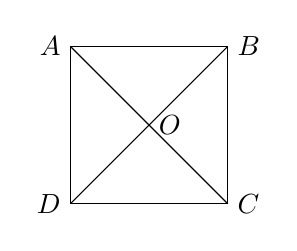
\begin{tikzpicture}
\draw (0,0) node[below,left] {$D$} -- (2,0) node[below,right] {$C$} -- (2,2) node[above,right] {$B$} -- (0,2) node[above,left] {$A$} -- cycle; 
\draw (0,0) -- (2,2);
\draw (0,2) -- (2,0);
\draw (1,1) node[right] {$O$};
\end{tikzpicture}\end{center}
\begin{enumerate}
 \item Quelle est la valeur de $p_0$ ?
 \item Déterminer une relation de récurrence entre $p_n$ et $p_{n+1}$.
 \item En déduire $p_n$ en fonction de $n$.
 \item Interpréter la limite de la suite $(p_n)_{n\in \N^*}$.
\end{enumerate}
\end{Exercice}

\corr \begin{enumerate}
\item Au temps 0, le pion est en A. Donc l'événement $E_0$ est l'évènement impossible. Ainsi, $p_0=\P(E_0)=0$.

\item Soit $n\in \N$. On sait que $(E_n, \overline{E_n})$ est un système complet d'événements. D'après la formule des probabilités totales, on a :
\begin{align*}
 \P(E_{n+1}) &= \P(E_n) \times \P_{E_n}(E_{n+1}) + \P(\overline{E_n}) \times \P_{\overline{E_n}}(E_{n+1})\\
 &= p_n \times 0 + (1-p_n) \times \frac 13
\end{align*}
car si le pion est en $O$, il ne peut y rester et s'il n'est pas en $O$, par équiprobabilité il a une probabilité d'être en $O$ au temps suivant de $\dis \frac 13 \cdot$ Ainsi, pour tout n $\in \N$, 
$$p_{n+1} = -\frac 13 p_n + \frac 13$$

\item La suite $(p_n)_{n \geq 0}$ est arithmético-géométrique et la méthode usuelle permet d'obtenir que pour tout entier $n \geq 0$,
$$ p_n = \frac 14 \l( 1 - \l(\frac{-1}{3}\r)^n\r) $$
\item On a $\dis -1 < \frac{-1}{3}<1$ donc 
$$\dis \lim_{n\to \pinf} \l(\frac{-1}{3}\r)^n = 0$$
Par somme et produit de limites, on a alors :
\[ \lim_{n\to \pinf} p_n = \frac 14 \]
Après un temps long, la probabilité que le pion soit en $O$ est proche de $ \dis \frac 14 \cdot$
\end{enumerate}

\begin{Exercice}{} Dans une zone d\'esertique, un animal erre entre trois points d'eau $A, B$ et $C.$
A l'instant $t=0,$ il se trouve au point $A.$

\noindent Quand il a \'epuis\'e l'eau du point o\`u il se trouve, il part avec \'equiprobabilit\'e rejoindre l'un des deux autres points d'eau.

\noindent L'eau du point qu'il vient de quitter se r\'eg\'en\`ere alors.


Soit $n\in\N.$ On note :

\begin{itemize}

\item[$\bullet$] $A_n$ l'\'ev\'enement \og l'animal est en $A$ apr\`es son $n$-i\`eme trajet \fg.


\item[$\bullet$] $B_n$ l'\'ev\'enement \og l'animal est en $B$ apr\`es son $n$-i\`eme trajet \fg.


\item[$\bullet$] $C_n$ l'\'ev\'enement \og l'animal est en $C$ apr\`es son $n$-i\`eme trajet \fg.

\end{itemize}

\noindent On pose aussi, $a_n=P(A_n), b_n=P(B_n)$ et $c_n=P(C_n).$



\begin{enumerate}

	\item 
	\begin{enumerate}
		\item Exprimer $a_{n+1}$ en fonction de $b_n$ et $c_n.$
		
		\item Exprimer de m\^eme $b_{n+1}$ et $c_{n+1}$ en fonction de $a_n, b_n$ et $c_n.$
		
	\end{enumerate}
	
	\item On consid\`ere $A=\left(\begin{array}{ccc}
	0 & 1/2 & 1/2\\
	1/2 & 0 & 1/2\\
	1/2 & 1/2 & 0\end{array}\right) \cdot$
	
	D\'eterminer une matrice $P$ inversible et une matrice $D$ diagonale telles que $D=P^{-1}AP.$
	
	
	\item Expliquer comment on pourrait obtenir explicitement $a_n$, $b_n$ et $c_n$ en fonction de $n.$
	
	
	
	
\end{enumerate}
\end{Exercice}

\corr \begin{enumerate}

	\item 
	\begin{enumerate}
		\item Soit $n \geq 0$. La famille $(A_n,B_n,C_n)$ est un système complet d'événements donc d'après la formule des probabilités totales :
\begin{align*}
a_{n+1} & = P(A_{n+1}) \\
& = P(A_n) P_{A_n}(A_{n+1}) +P(B_n) P_{B_n}(A_{n+1}) +P(C_n) P_{C_n}(A_{n+1}) \\
& = a_n \times 0 + b_n \times \dfrac{1}{2} + c_n \times \dfrac{1}{2} 
\end{align*}
car quand l'animal a \'epuis\'e l'eau du point o\`u il se trouve, il part avec \'equiprobabilit\'e rejoindre l'un des deux autres points d'eau. Ainsi,
$$ a_{n+1} =  \dfrac{b_n}{2} + \dfrac{c_n}{2}$$
		\item De même que dans la question précédente, on montre que pour tout entier $n \geq 0$,
$$ b_{n+1} =  \dfrac{a_n}{2} + \dfrac{c_n}{2}$$
et 
$$ c_{n+1} =  \dfrac{a_n}{2} + \dfrac{b_n}{2}$$
	\end{enumerate}
	
	\item Le calcul du polynôme caractéristique donne :
	$$ \chi_A(X) = (X-1)(X+1/2)^2$$
La méthode usuelle permet d'obtenir que :
\begin{itemize}
\item $((1,1,1))$ est une base de $E_1(A)$.
\item $((1,0,-1),(0,1,-1))$ est une base de $E_{-1/2}(A)$.
\end{itemize}
La formiule de changement de base implique que $A=PDP^{-1}$ où :
$$ P = \begin{pmatrix}
1 & 1 & 0 \\
1 & 0 & 1 \\
1 & -1 & -1 \\
\end{pmatrix}, \; D= \textrm{diag}(1,-1/2,-1/2)$$
et la méthode usuelle pour inverser une matrice permet d'obtenir :
$$ P^{-1} = \dfrac{1}{3} \begin{pmatrix}
1 & 1 & 1 \\
2 & -1 & -1 \\
-1 & 2 & -1 \\
\end{pmatrix}$$
\item Pour tout entier $n \geq 0$, posons : 
$$ X_n = \begin{pmatrix}
a_n \\
b_n \\
c_n \\
\end{pmatrix}$$
D'après la question $1$, on a $X_{n+1}=A X_n$ et on montre alors par récurrence que pour tout entier $n \geq 0$,
$$ X_n = A^n X_0$$
Or on a $A^n=PD^n P^{-1}$ et $D^n$ est facile à calculer car $D$ est diagonale.
\end{enumerate}

\begin{Exercice}{} On lance indéfiniment 3 dés équilibrés simultanément. Pour tout $n \geq 1$, on note $A_n$ l'évènement \og on obtient une triple 6 pour la première fois au $n$-ième tirage \fg . Déterminer $P(A_n)$ pour tout $n \geq 1$ et en déduire la probabilité d'obtenir au moins une fois un triple $6$.
\end{Exercice}

\corr Pour tout $n \geq 1$, on pose $B_n$ : \og On n'obtient pas un triple 6 lors du $n$-ième tirage \fg . Il est clair que pour tout $n \geq 1$, $P(B_n) = \dis \frac{6^3-1}{6^3} = \frac{215}{216}$ (nous sommes en situation d'équiprobabilité, il y a $6^3$ issues possibles quand on lance les trois dés et une seule nous permet d'avoir un triple $6$).

\medskip

\noindent On a $A_1=\overline{B_1}$ et donc 
$$P(A_1) = \dis \frac{1}{216}$$
et pour tout entier $n \geq 2$, 
$$A_n = \dis B_1 \cap B_2 \cap \cdots \cap B_{n-1} \cap \overline{B_n} = \dis \bigcap_{i=1}^{n-1} B_i \cap \overline{B_n}$$
Les lancers étant indépendants, on a alors :
\[ P(A_n) = P(\bigcap_{i=1}^{n-1} B_i \cap \overline{B_n}) = \prod_{i=1}^{n-1} P(B_i) \times P( \overline{B_n})\]
ce qui implique :
\[ P(A_n) = \bigg{(} \frac{215}{216} \bigg{)}^{n-1} \times \frac{1}{216} \]
Remarquons que cette formule est encore vraie pour $n=1$.

\medskip
\noindent Soit $A$ l'évènement \og on obtient au moins une fois un triple $6$ \fg . Alors $A$ est réalisé si et seulement si l'un des évènements $A_n$ est réalisé pour $n \geq 1$. On a donc 
$$A= \dis \bigcup_{n=1}^{+ \infty} A_n$$
De plus, les évènements $A_n$ (avec $n \geq 1$) sont deux à deux incompatibles. Par définition d'une probabilité, on a alors :
\[ P(A) = \sum_{n=1}^{+ \infty} P(A_n) = \frac{1}{216} \times \sum_{n=1}^{+ \infty} \bigg{(} \frac{215}{216} \bigg{)}^{n-1} \]
La convergence étant assurée par définition. On fait alors apparaître la somme d'une série géométrique :
\begin{align*}
P(A) & = \frac{1}{216} \times \frac{216}{215} \sum_{n=1}^{+ \infty} \bigg{(} \frac{215}{216} \bigg{)}^{n} \\
& = \frac{1}{215} \bigg{(} \frac{1}{1-\frac{215}{216}} - 1 \bigg{)} 
\end{align*}
car $-1 < \dis \frac{215}{216} < 1$. On a finalement :
\[ P(A) = \frac{1}{215} \times (216-1) = 1 \]

\begin{Exercice}{} On lance deux dés équilibrés jusqu'à ce que la somme des numéros obtenus soit un multiple de $5$. 
\begin{enumerate}
\item 
\begin{enumerate}
\item Soit $n \in \mathbb{N}^*$.  Donner la probabilité que l'épreuve s'arrête au $n$-ième lancer sur une somme égale à $5$ (on pourra noter $A_n$ cet évènement).
\item Donner la probabilité que l'épreuve s'arrête sur une somme égale à 5.
\end{enumerate}
\item Donner la probabilité que l'épreuve s'arrête par l'obtention d'un 10.
\item L'épreuve peut-elle ne jamais s'arrêter?
\end{enumerate}
\end{Exercice}

\corr \begin{enumerate}
\item 
\begin{enumerate}
\item Commençons par quelques remarques : quand on lance deux dés équilibrés, on est en situation d'équiprobabilité et le cardinal de l'univers est $36$. Les issues associées à l'obtention d'une somme égale à 5 sont $(1,4)$, $(4,1)$, $(2,3)$ et $(3,2)$. Ainsi la probabilité d'avoir une somme égale à $5$ est $\frac{4}{36} = \frac{1}{9}$ et de la même manière, la probabilité d'avoir une somme égale à $10$ est $\frac{3}{36} = \frac{1}{12}$ et finalement la probabilité d'obtenir une somme multiple de $5$ est $\frac{7}{36}$ (par incompatibilité).

\medskip

\noindent Notons pour tout entier $k \geq 1$, $B_k$ l'évènement \og On obtient une somme non multiple de $5$ lors du $k$-ième lancer \fg et distinguons deux cas :

\begin{itemize}
\item$P(A_1)= \dfrac{1}{9}$ (fait précédemment).
\item Pour tout entier $n \geq 2$, $A_n = B_1 \cap \cdots \cap B_{n-1} \cap A_n$ et d'après la formule des probabilités composées :
$$ P(A_n) = P(B_1) \times \cdots P_{B_1 \cap \cdots \cap B_{n-2}}(B_{n-1}) \times P_{B_1 \cap \cdots \cap B_{n-1}}(A_n)$$
et donc :
$$ \boxed{P(A_n) = \left( \frac{29}{36} \right)^{n-1}  \frac{1}{9}}$$
Remarquons que cette expression est valable pour $n=1$.
\end{itemize}
\item Notons $C$ cet évènement. On a $C = \bigcup_{k=1}^{+ \infty} A_k$ et ces évènements sont deux a deux incompatibles donc :
$$ P(C) = \sum_{k=1}^{+\infty} P(A_k)  = \frac{1}{9} \sum_{k=1}^{+\infty} \left( \frac{29}{36} \right)^{k-1} $$
par linéarité. On pose $j=k-1$ : si $k=1$, $j=0$ et si $k$ tend vers $+ \infty$, $j$ aussi donc :
$$ P(C) = \frac{1}{9}  \sum_{j=0}^{+\infty} \left( \frac{29}{36} \right)^{j}$$
On remarque la somme d'une série géométrique convergente car $\dfrac{29}{36} \in ]-1,1[$. On a donc :
$$P(C) = \frac{1}{9} \times \frac{1}{1-\frac{29}{36}} = \frac{1}{9} \times \frac{36}{7} = \frac{4}{7}$$
\end{enumerate}
\item De la même manière que précédemment, on obtient que la probabilité demandée vaut $\dfrac{3}{7}\cdot$
\item En pratique oui mais la somme des deux probabilités précédentes étant égale à $1$, la probabilité que cela arrive vaut $0$.
\end{enumerate}

\begin{Exercice}{} On lance une infinité de fois une pièce équilibrée. On note pour tout $n \in \mathbb{N}^*$, $A_n$ l'évènement \og on obtient au moins une fois la séquence pile pile face au cours des $n$ premiers lancers \fg et $P_n$  l'évènement \og on obtient pile au $n$-ième lancer \fg .

\begin{enumerate}
\item Donner $P(A_1)$, $P(A_2)$ et $P(A_3)$.
\item Soit $n$ un entier supérieur ou égal à 4.
\begin{enumerate}
\item Montrer que $A_{n+1} = A_n  \cup (\overline{A_{n-2}} \cap P_{n-1} \cap P_n \cap \overline{P_{n+1}})$.
\item En déduire un lien entre $P(A_{n+1})$, $P(A_n)$ et $P(A_{n-2})$. 
\item Montrer que la suite $(P(A_n))_{n \geq 4}$ est croissante. Est-elle convergente ? Si oui, donner sa limite.
\item Montrer que la famille d'évènements $(A_n)_{n \geq 0}$ est croissante. En déduire $\dis P \bigg{(} \bigcup_{n=1}^{+  \infty} A_n \bigg{)}$. Qu'en déduit-on ?
\end{enumerate}
\end{enumerate}
\end{Exercice}

\corr 

\begin{enumerate}
\item On a clairement :
$$ A_1=A_2= \varnothing$$
donc $P(A_1)=P(A_2)=0$. On a de plus :
$$ A_3 = P_1 \cap P_2 \cap \overline{P_3}$$
Par mutuelle indépendance, on en déduit que :
$$ P(A_3) = P(P_1) \times P(P_2) \times P(\overline{P_3}) = \dfrac{1}{8}$$
\item 
\begin{enumerate}
\item Raisonnons par double inclusion.
\begin{itemize}
\item Supposons que $A_{n+1}$ se réalise. Soit $A_n$ se réalise, soit $A_n$ ne se réalise pas : dans ce cas, la séquence pile pile face n'est pas obtenu lors des $n$ premiers lancers (en particulier lors des $n-2$ premiers). Nécessairement, la séquence pile pile face est obtenu lors des $n-1$, $n$ et $n+1$-ième lancers et ainsi $(\overline{A_{n-2}} \cap P_{n-1} \cap P_n \cap \overline{P_{n+1}})$ se réalise. Ainsi,
$$ A_{n+1} = A_n  \cup (\overline{A_{n-2}} \cap P_{n-1} \cap P_n \cap \overline{P_{n+1}})$$
\item Si $A_n$ se réalise, il est évident que $A_{n+1}$ se réalise donc :
$$ A_n \subset A_{n+1}$$
Si $(\overline{A_{n-2}} \cap P_{n-1} \cap P_n \cap \overline{P_{n+1}})$ se réalise, la séquence pile pile face est obtenu lors des $n+1$ premiers lancers donc $A_{n+1}$ se réalise. Ainsi,
$$ (\overline{A_{n-2}} \cap P_{n-1} \cap P_n \cap \overline{P_{n+1}}) \subset A_{n+1}$$
On en déduit que :
$$ A_n \cup (\overline{A_{n-2}} \cap P_{n-1} \cap P_n \cap \overline{P_{n+1}})\subset A_{n+1}$$
\end{itemize}
Par double inclusion, on en déduit que :
$$A_{n+1} = A_n  \cup (\overline{A_{n-2}} \cap P_{n-1} \cap P_n \cap \overline{P_{n+1}})$$
\item Soit $n \geq 4$. Les événements :
$$  A_n  \; \hbox{ et } \;  (\overline{A_{n-2}} \cap P_{n-1} \cap P_n \cap \overline{P_{n+1}})$$
sont incompatibles. En effet, si l'on suppose qu'ils se réalisent simultanément alors on obtient pile pile aux $n-1$ et $n$-ièmes lancers et on obtient la séquence pile pile face lors des $n$ premiers lancers et donc nécessairement lors des $n-2$ premiers (car les deux derniers sont des piles). Ainsi, $A_{n-2}$ se réalise ce qui est faux car $\overline{A_{n-2}}$ se réalise. Ainsi, par incompatibilité et d'après la question précédente :
$$ P(A_{n+1}) = P(A_n) +   P(\overline{A_{n-2}} \cap P_{n-1} \cap P_n \cap \overline{P_{n+1}})$$
Les lancers étant indépendants et l'évènement $\overline{A_{n-2}}$ ne dépendant que des $n-2$ premiers, on en déduit que :
\begin{align*}
P(A_{n+1}) & = P(A_n) +   P(\overline{A_{n-2}}) \times P( P_{n-1}) \times P(P_n) \times P(\overline{P_{n+1}}) \\
& = P(A_n) + \dfrac{1}{8} (1-P(A_n))
\end{align*}
\item Soit $n \geq 4$. D'après la question précédente :
$$ P(A_{n+1})-P(A_n)= \dfrac{1}{8} (1-P(A_n)) \geq 0$$
car $P(A_n) \in [0,1]$. Ainsi, $(P(A_n))_{n \geq 4}$ est croissante. Cette suite est aussi majorée par $1$ donc elle converge vers un réel $\ell$. Par passage à la limite dans l'égalité obtenue dans la question précédente, on a :
$$ \ell = \ell + \dfrac{1}{8}(1- \ell)$$
donc $\ell =1$.
\item Soit $n \geq 0$. Si $A_{n}$ se réalise, la séquence pile pile face est obtenu lors des $n$ premiers lancers donc en particulier lors des $n+1$ premiers lancers et ainsi, $A_{n+1}$ se réalise. Ainsi, $(A_n)_{n \geq 0}$ est croissante. Par continuité croissante, on en déduit que :
$$\dis P \bigg{(} \bigcup_{n=1}^{+  \infty} A_n \bigg{)} = \lim_{n \rightarrow + \infty} P(A_n) = 1$$
On en déduit que l'évènement $\bigcup_{n=1}^{+  \infty} A_n $ se réalise avec probabilité $1$. Ainsi, presque-surement, on obtient la séquence pile pile face.
\end{enumerate}
\end{enumerate}

\begin{Exercice}{}
Soit $p \in ]0,1[$. On note $q=1-p$.\\
On effectue une infinité de lancers indépendants d'une pièce pour laquelle la probabilité d'obtenir Face est $p$.
\begin{enumerate}
\item Pour tout $n \in \mathbb{N}^*$, on note $A_n$ l'événement \og Au cours des $n$ premiers lancers, Face n'est jamais suivi de Pile\fg.
Montrer que :
$$P(A_n)=\begin{cases}
{\frac{p^{n+1}-q^{n+1}}{p-q}} & \text{si } p \neq \frac 1 2\\
{\frac{n+1}{2^n}} & \text{si } p=\frac 1 2
\end{cases}$$
\item Est-il possible que Face ne soit jamais suivi de Pile ?\\
Calculer la probabilité de l'événement $A$ : \og Face n'est jamais suivi de Pile \fg.
\end{enumerate}
\end{Exercice}

\corr Notons pour tout entier $k \geq 1$, $F_k$ l'événement \og La pièce donne face lors du $k$-ième lancer \fg .

\begin{enumerate}
\item Soit $n \in \mathbb{N}^*$. L'évènement $A_n$ se réalise si et seulement si l'un de ces évènements (qui sont deux à deux incompatibles) se réalisent :
\begin{itemize}
\item On obtient que des piles lors des $n$ premiers lancers.
\item On obtient que des piles lors des $n-1$ premiers lancers puis face au $n$-ième lancer.
\item On obtient que des piles lors des $n-2$ premiers lancers puis face au lors des $n-1$-ième et $n$-ième lancer.
\item $\ldots$
\item On obtient que des faces lors des $n$ premiers lancers.
\end{itemize}
Ainsi,
$$ A_n =\bigcup_{k=0}^n (\overline{F_1} \cap \cdots \cap \overline{F_k}) \cap (F_{k+1} \cap \cdots \cap F_n)$$
puis par incompatibilité :
$$ P(A_n) = \sum_{k=0}^n P( (\overline{F_1} \cap \cdots \cap \overline{F_k}) \cap (F_{k+1} \cap \cdots \cap F_n))$$
et par indépendance des lancers :
\begin{align*}
 P(A_n) & = \sum_{k=0}^n P(\overline{F_1}) \times \cdots \times P(\overline{F_k}) \times P(F_{k+1}) \times \cdots \times P( F_n) \\
 & = \sum_{k=0}^n  (1-p)^k p^{n-k} \\
 & = p^{n} \sum_{k=0}^n \left( \dfrac{1-p}{p} \right)^k 
 \end{align*}
Remarquons maintenant que :
$$\dfrac{1-p}{p} = 1 \Longleftrightarrow 1-p=p \Longleftrightarrow 2p=1 \Longleftrightarrow p = \dfrac{1}{2}$$
Ainsi, si $p = \dfrac{1}{2}$,
$$ P(A_n) = \dfrac{1}{2^{n}} \sum_{k=0}^n 1 = \dfrac{n+1}{2^{n+1}}$$
Si $p \neq 1$, par somme des termes d'une suite géométrique, on a :
\begin{align*}
P(A_n) & = p^n \dfrac{1-((1-p)/p)^{n+1}}{1-(1-p)/p} \\
& = p^{n+1} \dfrac{1-((1-p)/p)^{n+1}}{p-(1-p)} \\
& = \dfrac{p^{n+1}-(1-p)^{n+1}}{p-(1-p)} \\
& = \dfrac{p^{n+1}-q^{n+1}}{p-q}
\end{align*}
\item A priori, oui c'est possible si l'on obtient que des faces ou que des piles. 

\medskip

\noindent L'évènement $A$ se réalise si et seulement pour tout entier $n \geq 1$, au cours des $n$ premiers lancers, face n'est jamais suivi de pile. Ainsi,
$$ A = \bigcap_{n=1}^{+ \infty} A_n$$
Pour tout $n \geq 1$, si $A_{n+1}$ se réalise alors au cours des $n+1$ premiers lancers, face n'est jamais suivi de pile et en particulier au cours $n$ premiers lancers, face n'est jamais suivi de pile donc $A_n$ se réalise. Ainsi, $A_{n+1} \subset A_n$ donc $(A_n)_{n \geq 1}$ est décroissante. Par continuité décroissante, on en déduit que $(P(A_n))_{n \geq 1}$ converge et :
$$ P(A) = \lim_{n \rightarrow + \infty} P(A_n)$$
Sachant que $p$ et $q$ appartient à $]0,1[$ si $p \neq 1/2$ et en utilisant le théorème des croissances comparées si $p=1/2$, on en déduit que :
$$ P(A)=0$$
\end{enumerate}

\begin{Exercice}{} Un enfant lance un galet pour faire des ricochets sur l'eau. On suppose que la probabilité que le galet ricoche pour la $n$-ième fois sachant qu'il a ricoché les $(n-1)$ coups d'avant, est égale à $\dis \frac{1}{n}\cdot$ On suppose que lors du premier coup, le galet ricoche nécessairement.
\begin{enumerate}
\item Soit $n \in \mathbb{N}^*$. Déterminer la probabilité $p_n$ que le galet coule après $n$ ricochets réussis.
\item Montrer que $\dis \sum_{n \geq 1} p_n$ converge, donner sa somme et interpréter.
\end{enumerate}
\end{Exercice}

\corr Notons pour tout entier $k \geq 1$, $A_k$ l'évènement \og Le galet ricoche au $k$-ième coup \fg.

\begin{enumerate}
\item Soit $n \geq 1$. On a :
$$ p_n = \P(A_1 \cap A_2 \cap \cdots \cap A_n \cap \overline{A_{n+1})}$$
D'après la formule des probabilités composées, sachant que la probabilité de $A_1 \cap A_2 \cap \cdots \cap A_n $ est non nulle, on a :
\begin{align*}
p_n & = \P(A_1) \P_{A_1}(A_2) \times \cdots \times \P_{A_1 \cap \cdots \cap A_{n-1}}(A_n) \times \P_{A_1 \cap \cdots \cap A_{n}}(\overline{A_{n+1}}) \\
& = 1 \times \dfrac{1}{2} \times \cdots \times \dfrac{1}{n} \times \left(1- \dfrac{1}{n+1} \right) \\
& = \dfrac{1}{n!} \left(1- \dfrac{1}{n+1} \right) \\
& = \dfrac{1}{n!} - \dfrac{1}{(n+1)!}
\end{align*}
\item Pour tout entier $N \geq 1$,
\begin{align*}
\sum_{k=1}^N p_k & = \sum_{k=1}^N \dfrac{1}{k!} - \dfrac{1}{(k+1)!} \\
& = 1- \dfrac{1}{(N+1)!}
\end{align*}
On a :
$$ \lim_{N \rightarrow + \infty}  1- \dfrac{1}{(N+1)!} = 1$$
Ainsi, $\dis \sum_{n \geq 1} p_n$ converge et sa somme vaut $1$.

\medskip

\noindent Notons pour tout entier $n \geq 1$, $B_n$ l'évènement \og Le galet ricoche $n$ fois avant de couler \fg et $B$ l'évènement \og Le galet coule \fg{}. Alors on a :
$$ B = \bigcup_{n=1}^{+ \infty} B_n$$
Les évènements $B_n$ étant deux à deux incompatibles, on en déduit que :
$$ \P(B) = \sum_{n=1}^{+ \infty} \P(B_n) =  \sum_{n=1}^{+ \infty} p_n = 1$$
Ainsi, le galet coule presque-surement.
\end{enumerate}

\begin{Exercice}{} On effectue une succession infinie de lancers indépendants d'une pièce
donnant Pile avec la probabilité $p\in ]0,1[$ et Face avec la probabilité $%
q=1-p$.\newline
On s'intéresse dans cet exercice aux successions de lancers amenant un mê%
me côté.\newline
On dit que la première série est de longueur $n\geq 1$ si les $n$
premiers lancers ont amené le même côté de la pièce et le $(n+1)$-ième
l'autre côté.\newline
De même la deuxième série commence au lancer suivant la fin de la première sé%
rie et se termine (si elle se termine) au lancer précédant un changement de c%
ôté.\newline


\begin{enumerate}
\item Pour tout $n \in \mathbb{N}^*$, on note $A_n$ l'évènement \og La longueur de la première série est égale à $n$ \fg. Déterminer $P(A_n)$.
\item Montrer que :
\[\sum\limits_{n=1}^{+\infty }P(A_n)=1\]
Quelle est la probabilité que la première série ne se termine pas?

\item Pour $n \in \mathbb{N}^*$, on note $B_n$ l'évènement \og La longueur de la deuxième série est égale à $n$ \fg .

\begin{enumerate}
\item Déterminer pour $(n,k) \in (\mathbb{N}^*)^2$, $P(A_n \cap B_k)$.

\item En déduire que, pour $k\in \mathbb{N}^{* }$, $P(B_k)$.
\end{enumerate}
\end{enumerate}
\end{Exercice}

\corr Pour tout $i\in \mathbb{N}^{* }$, on note $P_{i}$ l'événement \og le $i$-ième lancer amène Pile \fg.

\begin{enumerate}
\item Soit $n \in \mathbb{N}^*$. L'évènement $A_n$ est réalise si et seulement si on obtient lors des $n$ premiers lancers Pile puis Face au $(n+1)$-ième lancer ou si on  obtient lors des $n$ premiers lancers Face puis Pile au $(n+1)$-ième lancer. Ainsi 
\[ A_n = \left( \bigcap_{i=1}^n P_i \bigcap \overline{P_{n+1}} \right) \cup \left( \bigcap_{i=1}^n \overline{P_i} \bigcap P_{n+1} \right)\]
Alors 
\[ \begin{array}{llll}
P(A_n) & = & \dis P\left(\left( \bigcap_{i=1}^n P_i \bigcap \overline{P_{n+1}} \right) \cup \left( \bigcap_{i=1}^n \overline{P_i} \bigcap P_{n+1} \right)\right) & \\
& = &  \dis P\left(\bigcap_{i=1}^n P_i \bigcap \overline{P_{n+1}}\right) + P  \left(\bigcap_{i=1}^n \overline{P_i} \bigcap P_{n+1} \right) & \hbox{(incompatibilité)} \\
& = & \dis \prod_{i=1}^n P(P_i) \times P( \overline{P_{n+1}}) + \prod_{i=1}^n P(\overline{P_i}) \times P( P_{n+1}) & \hbox{(indépendance des lancers)} \\
& = & p^n q + q^n p \\
\end{array} \]
\item Étudions les sommes partielles de cette série. Soit $N \geq 1$, on a :
\[ \begin{array}{ccl}
\dis \sum_{n=1}^N P(A_n) & = & \dis \sum_{n=1}^N p^nq + q^np \\
 & = & q \dis \sum_{n=1}^N p^n + p \dis \sum_{n=1}^N q^n \\
 \end{array} \]
 On reconnait les sommes partielles de séries géométriques convergentes car $p,q \in ]0,1[$. La série de terme général $P(A_n)$ est donc convergente et on a :
 \[ \sum_{n=1}^{ + \infty} P(A_n)  = q \sum_{n=1}^{+ \infty} p^n +p \sum_{n=1}^{+ \infty} q^n = q \left( \frac{1}{1-p} - 1 \right) +  p \left( \frac{1}{1-q} - 1 \right) \]
Or $q=1-p$, on a donc :
 \[   \sum_{n=1}^{ + \infty} P(A_n) = (1-p) \times \frac{1-(1-p)}{1-p} + p \times \frac{1-p}{p} = 1-(1-p)+1-p=1 \]
Soit $C$ l'évènement \og La première série ne se termine pas \fg . L'évènement contraire de $C$ est réalisé si et seulement l'un des évènements $A_n$ est réalisé pour $n \geq 1$. Ainsi,
\[ \overline{C} = \bigcup_{i=1}^{+ \infty} A_i \]
Ainsi 
$$P(\overline{C})= P \dis \left(\bigcup_{i=1}^{+ \infty} A_i \right) = \sum_{n=1}^{+  \infty} P(A_n)$$
par deux à deux incompatibilité des évènements et finalement $P(\overline{C})=1$. Ainsi, $P(C)=0$.
\item 
\begin{enumerate}
\item De la même manière que dans la question 1. on a :
\[ A_n \cap B_k = \left( \bigcap_{i=1}^n P_i \bigcap \bigcap_{i=n+1}^{n+k} \overline{P_i} \bigcap P_{n+1} \right) \bigcup \left( \bigcap_{i=1}^n \overline{P_i} \bigcap \bigcap_{i=n+1}^{n+k} P_i \bigcap \overline{P_{n+1}} \right) \]
Avec les mêmes justifications que dans la question 1. on obtient :
\[ P(A_n) = p^n \times q^k \times p + q^n \times p^k \times q = p^{n+1} q^k + q^{n+1} p^k \]
\item Les évènements $A_n$ ($n \geq 1$) et l'évènement $C$ forment un système complet d'évènements (soit la série s'arrête après un lancer, après deux lancers, \ldots ou ne se termine jamais). En utilisant que $P(C)=0$ et d'après la formule des probabilités totales, on a pour tout $k \geq 1$,
\[ P(B_k) = \sum_{n=1}^{+ \infty} P(A_n \cap B_k) = \sum_{n=1}^{\infty} p^{n+1} q^k + q^{n+1} p^k \]
Considérons une somme partielle de cette série convergente (d'après la formule des probabilités totales). Soit $N \geq 1$, on a :
\[ \sum_{n=1}^N p^{n+1} q^k +q^{n+1} p^k = q^k \sum_{n=1}^N p^{n+1} + p^k \sum_{n=1}^N q^{n+1} \]
ce qui implique que 
\[ \sum_{n=1}^N p^{n+1} q^k +q^{n+1} p^k = p^2 q^k \sum_{n=1}^N p^{n-1} + q^2p^k \sum_{n=1}^N q^{n-1} \]
Par changement d'indice, on a :
\[ \sum_{n=1}^N p^{n+1} q^k +q^{n+1} p^k = p^2 q^k \sum_{j=0}^{N-1} p^{j} + q^2p^k \sum_{j=0}^{N-1} q^{j} \]
On fait tendre $N$ vers $+\infty$ (on reconnait les sommes partielles de séries géométriques convergentes car $p,q \in ]0,1[$) ce qui donne :
\[ P(B_k) = p^2 q^k \times \frac{1}{1-p} + q^2 p^k \times \frac{1}{1-q} = p^2 q^{k-1} + q^2 p^{k-1} \]
car $p=1-q$.
\end{enumerate}
\end{enumerate}

\medskip

\begin{center}
\textit{{ {\large Divers}}}
\end{center}

\medskip


\begin{Exercice}{} Soit $(A_n)_{n \geq 0}$ une famille d'évènements mutuellement indépendants d'un même espace probabilisé.
\begin{enumerate}
\item On suppose que $\dis \sum_{n \geq 0} P(A_n)$ converge. Montrer que :
$$ \P \left( \bigcap_{n \geq 0} \overline{A_n} \right) \leq \exp \left(- \sum_{k=0}^{+ \infty} \P(A_k) \right)$$
\item On suppose que $\dis \sum_{n \geq 0} P(A_n)$ diverge. Montrer que :
$$ \P \left( \bigcap_{n \geq 0} \overline{A_n} \right) = 0$$
\end{enumerate}
\end{Exercice}

\corr 
\begin{enumerate}
\item Soit $N \geq 0$. Les évènements $A_n$ ($n \geq 0$) sont mutuellement indépendants donc les évènements $\overline{A_n}$ aussi. Ainsi,
$$  P \left( \bigcap_{k=0}^N \overline{A_k} \right) = \prod_{k=0}^N P( \overline{A_k}) =  \prod_{k=0}^N 1- P(A_k) $$
On sait que pour tout réel $y$,
$$ 1+y \leq e^y$$
donc pour tout réel $x$,
$$ 1-x \leq e^{-x}$$
En appliquant cette inégalité avec $x=P(A_k)$ et sachant que $1-P(A_k)$ est un terme positif, on en déduit que :

\begin{align*}
P \left( \bigcap_{k=0}^N \overline{A_k} \right) & = \prod_{k=0}^N 1- P(A_k) \\
& \leq \prod_{k=0}^N e^{-P(A_k)} \\
& = \exp \left(- \sum_{k=0}^N P(A_k) \right)
\end{align*}
On sait que :
$$ \lim_{N \rightarrow + \infty} \sum_{k=0}^N P(A_k) = \sum_{k=0}^{+ \infty} P(A_k)$$
donc par continuité de l'exponentielle sur $\mathbb{R}$ :
$$ \lim_{N \rightarrow + \infty}\exp \left(- \sum_{k=0}^N P(A_k) \right) = \exp \left(- \sum_{k=0}^{+ \infty} P(A_k) \right)$$
D'après l'application (faite en cours) de théorème de continuité croissante/décroissante, on sait que :
$$ \lim_{N \rightarrow + \infty} P \left( \bigcap_{k=0}^N \overline{A_k} \right) = P \left( \bigcap_{k=0}^{+ \infty} \overline{A_k} \right)$$
Ainsi, par passage à la limite dans l'inégalité obtenue précédemment, on en déduit que :
$$ P \left( \bigcap_{k=0}^{+ \infty} \overline{A_k} \right) \leq \exp \left(- \sum_{k=0}^{+ \infty} P(A_k) \right)$$
\item On sait que pour tout entier $N \geq 0$,
$$ 0 \leq P \left( \bigcap_{k=0}^N \overline{A_k} \right) \leq \exp \left(- \sum_{k=0}^N P(A_k) \right)$$ 
La série à termes positifs $\dis \sum_{n \geq 0} P(A_n)$ diverge donc :
$$ \lim_{N \rightarrow + \infty} \sum_{k=0}^N P(A_k) = + \infty$$
donc par composition avec l'exponentielle :
$$ \lim_{N \rightarrow + \infty}\exp \left(- \sum_{k=0}^N P(A_k) \right) =0$$
Par théorème d'encadrement, on en déduit que :
$$ \lim_{N \rightarrow + \infty} P \left( \bigcap_{k=0}^N \overline{A_k} \right) = 0$$
D'après l'application (faite en cours) de théorème de continuité croissante/décroissante, on sait que :
$$ \lim_{N \rightarrow + \infty} P \left( \bigcap_{k=0}^N \overline{A_k} \right) = P \left( \bigcap_{k=0}^{+ \infty} \overline{A_k} \right)$$
On en déduit par unicité de la limite que :
$$ P \left( \bigcap_{k=0}^{+ \infty} \overline{A_k} \right) = 0$$
\end{enumerate}

\begin{Exercice}{} Soit $(A_n)_{n \geq 0}$ une suite d'évènements d'un même espace probabilisé ayant tous probabilité 1. 
 
 \begin{enumerate}
 \item Montrer que $\P \left( \bigcup_{n \geq 0} \overline{A_n} \right) = 0$.
 \item Qu'en déduit-on pour $\P \left( \bigcap_{n \geq 0} A_n \right)$?
 \end{enumerate}
 \end{Exercice}
 
 \corr 
 
 \begin{enumerate}
 \item La série de terme général $\P( \overline{A_n})$ converge (tous les termes sont nuls car pour tout $n \geq 0$, $\P( \overline{A_n})= 1- \P(A_n)=0$) donc :
 $$ 0 \leq \P \left( \bigcup_{n \geq 0} \overline{A_n} \right) \leq \sum_{n=0}^{+ \infty} \P( \overline{A_n})  = \sum_{n=0}^{+ \infty} 0 = 0$$
 Ainsi,
 $$ \P \left( \bigcup_{n \geq 0} \overline{A_n} \right)=0$$
 \item D'après les lois de Morgan, on a :
 \begin{align*}
 \P \left( \bigcap_{n \geq 0} A_n \right) & = 1 - \P \left( \overline{\bigcap_{n \geq 0} A_n} \right) \\
 &= 1 - P \left( \bigcup_{n \geq 0} \overline{A_n} \right) \\
 & =1-0 \\
 & = 1
 \end{align*}
 \end{enumerate}
\end{document}